% =====================================================================
% Bias-corrected estimation of the interventional outcome density under
% a continuous, multidimensional treatment, with an MCD nuisance.
%
% Notation follows the companion MCD paper:
%   mixture ratio        pi          (\ratio)
%   contrast function    D_pi        (\contrast)
%   density ratio        R           (\DensityRatio)
%   augmented pair       (W,Z),  W=(T,X,Y)
%   densities            f_{...}     (\pf{...})
% The generalized propensity score is written e(t|x) to avoid colliding
% with the mixture ratio; the score displacement of the classifier is
% written S(w;beta) to avoid colliding with the contrast function.
% =====================================================================

\documentclass[11pt]{article}

\usepackage[T1]{fontenc}
\usepackage[margin=1in]{geometry}
\usepackage{amsmath,amssymb,amsthm}
\usepackage{bm}
\usepackage{relsize}
\usepackage{dsfont}
\usepackage{mathtools}
\usepackage{hyperref}
\usepackage[round]{natbib}
\usepackage{parskip}
\usepackage{booktabs}
\usepackage{array}
\usepackage{algorithm}
\usepackage{algpseudocode}

\theoremstyle{plain}
\newtheorem{theorem}{Theorem}
\newtheorem{mypropo}{Proposition}
\newtheorem{lem}{Lemma}
\newtheorem{corollary}{Corollary}
\theoremstyle{definition}
\newtheorem{mydef}{Definition}
\newtheorem{assumption}{Assumption}
\theoremstyle{remark}
\newtheorem{remark}{Remark}

% ---- subset of 00_Notations.tex ----
\newcommand{\ourmethod}{\text{MCD}\,}
\newcommand{\mcd}{\text{MCD}\,}
\newcommand{\MCF}{\ensuremath{\text{MCFunct}}}
\newcommand{\MDC}{\ensuremath{\text{MDCond}}}
\newcommand{\pE}{\ensuremath{\mathbb{E}}}
\newcommand{\pP}{\ensuremath{\mathbb{P}}}
\newcommand{\Var}{\mathbb{V}\text{ar}}
\newcommand{\R}{\mathbb{R}}
\newcommand{\cW}{\ensuremath{\mathcal{W}}}
\newcommand{\cX}{\ensuremath{\mathcal{X}}}
\newcommand{\cY}{\ensuremath{\mathcal{Y}}}
\newcommand{\cT}{\ensuremath{\mathcal{T}}}
\newcommand{\cR}{\ensuremath{\mathcal{R}}}
\newcommand{\pf}[1]{\ensuremath{\,\mathlarger{\textit{f}}_{#1}}}
\newcommand{\pfhat}[1]{\ensuremath{\,\mathlarger{\widehat{\textit{f}}}_{#1}}}
\newcommand{\ratio}{\ensuremath{\pi}}
\newcommand{\contrast}{D_{\ratio}}
\newcommand{\contrasthat}{\widehat{D}_{\mcd}}
\newcommand{\DensityRatio}{\text{R}}
\newcommand{\mDwz}[1]{\ensuremath{\mathcal{D}}_{#1}^{W,Z}}
\newcommand{\betahat}{\widehat{\beta}}
\newcommand{\Indi}{\ensuremath{\mathds{1}}}
\newcommand{\ks}{k}
\newcommand{\cO}{\mathcal{O}}

% ---- specific to this paper ----
\newcommand{\dd}{\,\mathrm{d}}
\newcommand{\IF}{\mathrm{IF}}
\newcommand{\gps}{e}
\newcommand{\score}{S}
\newcommand{\Rem}{\mathrm{Rem}}

\usepackage{tikz}
\usetikzlibrary{positioning, arrows.meta}
\tikzset{
    dagnode/.style={circle, draw, thick, minimum size=1cm},
    dagarrow/.style={-{Latex[length=3mm,width=2mm]}, thick}
}

\title{Bias-Corrected Estimation of the Interventional Density\\
Under a Continuous, Multidimensional Treatment}
\author{}
\date{}

\begin{document}
\maketitle

\begin{abstract}
We study the estimation of the interventional density of a scalar outcome under a
continuous, possibly multidimensional treatment. Under the back-door adjustment, this
target reduces to a single conditional density whose conditioning set contains the
treatment and every confounder, and which is therefore high-dimensional while the outcome
is scalar. Marginal contrastive discrimination is tailored to this asymmetry: it replaces
the conditional density by a univariate marginal and a binary classifier, so that no
density on a high-dimensional space is ever fitted. The resulting plug-in estimator,
however, inherits a first-order bias. Removing that bias by the standard one-step
correction requires the influence function of the target, which contains the generalized
propensity score --- itself a conditional density in the treatment, and precisely the
object the contrastive construction was meant to avoid. Our main contribution is to
re-express the same correction through the contrastive factorization. The generalized
propensity score then disappears from the formula; in exchange, the correction now requires
the influence function of the fitted contrast function, whose training sample is built from
the data and which therefore behaves unlike the influence function of an ordinarily trained
model. We compute this influence function in closed form for a penalized logistic contrast,
assemble the corrected estimator, and prove its asymptotic normality with a closed-form
variance.
\end{abstract}

\section{Introduction}
\label{sec:intro}

A prediction describes what is likely to happen; a causal statement describes what would
happen under an intervention. Decisions call for the second. A clinician choosing a dose, a
regulator setting an exposure limit, and an analyst evaluating a policy all need the
distribution of an outcome under an intervention. Randomized experiments answer such
questions by construction, but they are often unavailable, and the causal quantity must then
be recovered from observational data, in which the treatment is chosen rather than assigned
and the reasons for the choice usually affect the outcome as well.

Most of the causal-inference literature reports a mean: the average treatment effect or, for
a treatment ranging over a continuum, the dose-response curve $t \mapsto \pE[Y(t)]$, where
$Y(t)$ is the potential outcome under treatment level $t$. A mean, however, collapses a
distribution to a single number, and two interventions with equal means may induce very
different outcome distributions. Whenever the question concerns the probability of exceeding
a threshold, the spread of the response, or any functional of the outcome law beyond its
first moment, the relevant object is the full interventional density
\[
p_t(y) = \pf{Y(t)}(y),
\]
the density of $Y(t)$ at the point $y$. Its semiparametric theory in the discrete-treatment
case is due to \citet{kennedy2023density}, who derived the efficient influence function and
a doubly robust estimator; alternative discrete-treatment estimators, differing in how the
density is represented, were given by \citet{melnychuk2023flows},
\citet{ham2024logconcave} and \citet{martinez2023stein}. All of these assume a treatment
with finitely many levels.

This paper treats the continuous case, which is both more common in applications and harder
in theory. Doses, durations, concentrations and continuous policy instruments are not
naturally discretized, and applications often involve several such quantities at once, so
the treatment is a vector $T \in \cT \subseteq \R^d$. With a continuous treatment the
propensity score becomes the \emph{generalized} propensity score of \citet{imbens2000} and
\citet{hirano2004}, a conditional density in $t$ rather than a probability, and the target
is no longer estimable at the parametric rate: \citet{kennedy2017continuous} showed that the
dose-response curve requires smoothing in the treatment argument, and \citet{colangelo2020}
gave the corresponding debiased machine-learning estimator. In that line of work the target
has remained the mean. Here we keep the treatment continuous but take the target to be the
density.

Our identification rests on the back-door adjustment of \citet{pearl1995,pearl2009}, which
expresses the target as the conditional outcome density averaged over the covariates,
\[
p_t(y) = \pE_X\big[\pf{Y \mid T=t,X}(y)\big].
\]
Estimation therefore reduces to a single conditional density, evaluated at the treatment
level $t$ and averaged over the covariate distribution. This is where the difficulty
concentrates. The conditioning set is the pair $(T,X)$: it holds the treatment and every
confounder, and is high-dimensional, whereas the outcome is scalar. Standard nonparametric
conditional-density estimators are poorly suited to that asymmetry, because their rates
deteriorate with the dimension of the conditioning argument
\citep{stone1980,Tsybakov2009NonparametricEstimation}, and this rate governs the error of
the whole procedure.

Marginal contrastive discrimination \citep{meziani2025mcd} is designed for exactly this
asymmetry. It writes the conditional density as a univariate marginal times a density ratio,
and estimates the ratio by a binary classifier that separates observed vectors from vectors
whose outcome has been resampled from its own marginal. No density on a high-dimensional
space is ever fitted: the marginal is univariate, and the ratio is recovered by
classification, a problem any supervised learner can solve. The same principle underlies
noise-contrastive estimation \citep{gutmann2010nce} and classification-based density-ratio
estimation \citep{sugiyama2012density}, on which the contrastive construction builds.

Plugging this estimate into the back-door average yields an estimator of $p_t(y)$, but, like
every plug-in built on a nonparametric nuisance, it is biased at first order: the bias
equals the covariate average of the conditional-density error and vanishes only as slowly as
that error \citep{bickel1988,robins2008}. The standard remedy is the one-step correction of
semiparametric theory \citep{vanderlaan2006tmle,chernozhukov2018,kennedy2022review}, which
adds the empirical average of the target's influence function and renders the estimator
first-order insensitive to the nuisance. That correction, however, runs into a problem specific to our target. The influence function
of $p_t(y)$ contains the generalized propensity score: a second nuisance, and a conditional
density in the treatment coordinate --- exactly the object the contrastive construction was
adopted to avoid. Written in the usual way, the correction gives back the difficulty the
estimator was meant to remove.

The resolution exploits a basic fact about influence functions. The influence function of a
target is unique, but the target itself admits several equivalent expressions, and
differentiating any of them yields an equal --- though differently written --- formula for
the same object. We differentiate the target in its \emph{contrastive} form rather than its
back-door form. In that form the generalized propensity score never appears. The price is a
new object, the influence function of the fitted contrast function, which behaves unlike the
influence function of an ordinarily trained model because the contrastive training sample is
itself built from the data.

\paragraph{Contributions.}
The paper makes three contributions, in increasing order of technical novelty.
\begin{enumerate}
\item[(C1)] \emph{An influence function for the interventional density under a continuous
treatment.} We derive the nonparametric influence function of $p_t(y)$
(Proposition~\ref{prop:eif}). It carries a point mass in the treatment and a point mass in
the outcome, and recovers the known discrete-treatment and dose-response influence functions
as limiting cases. To our knowledge it has not appeared before for a continuous treatment
with a pointwise density target.
\item[(C2)] \emph{A correction that avoids the generalized propensity score.} We recompute
the same correction through the contrastive factorization (Proposition~\ref{prop:if-mcd}) and
find that the generalized propensity score is absent from it, the conditional outcome density
entering only through its two contrastive factors. This is the paper's central result: it
removes the second treatment-coordinate density that the classical correction reintroduces.
\item[(C3)] \emph{The influence function of a contrastively fitted classifier.} Because the
negative class is generated from the data, perturbing the law perturbs the training
distribution, and the influence function of the fitted contrast function is not the usual
sandwich formula: it has three score channels rather than one (Theorem~\ref{thm:channels}).
We compute them in closed form for a penalized logistic contrast, assemble the corrected
estimator, and establish its asymptotic normality with a closed-form variance
(Theorem~\ref{thm:asymptotics}).
\end{enumerate}

\paragraph{Organization.}
Section~\ref{sec:setting} fixes the setting, recalls the contrastive conditional-density
estimator, and isolates the first-order bias of the plug-in. Section~\ref{sec:eif} derives
the influence function and the corrected estimator, and identifies the cost of the
generalized propensity score it contains. Section~\ref{sec:mcd-correction} recomputes the
correction through the contrastive factorization, forms the corrected estimator, then computes
the contrast influence function --- in general and for the penalized logistic case --- and
establishes the limiting distribution.
Section~\ref{sec:discussion} discusses the procedure and its diagnostics. All derivations are
in the appendix, and each result in the body carries an explicit pointer to its proof.

\section{Setting}
\label{sec:setting}

This section fixes the estimand and the ingredients used to estimate it. We first record the
causal assumptions under which the interventional density is identified from observational
data, then recall the contrastive estimator of the conditional density on which the plug-in
rests, and finally show that this plug-in is biased at first order. That bias is the object
the remainder of the paper is devoted to removing.

\subsection{Notation}
\label{sec:setting-notation}

Let $T \in \cT \subseteq \R^{d}$ be a treatment, $X \in \cX \subseteq \R^{p}$ a vector of
covariates and $Y \in \cY \subseteq \R$ a scalar outcome. We observe $n$ independent copies
of
\[
W = (T,X,Y) \in \cW = \cT \times \cX \times \cY , \qquad W \sim F,
\]
and assume $F$ has a density with respect to Lebesgue measure. Following
\citet{meziani2025mcd}, we write $\pf{T,X,Y}$, $\pf{T,X}$, $\pf{X}$, $\pf{Y}$ for the joint
and marginal densities and $\pf{Y \mid T=t,X=x}$ for the conditional density of the outcome.
For $t \in \cT$, let $Y(t)$ be the potential outcome under the intervention setting the
treatment to $t$.

\subsection{Causal structure and identification}
\label{sec:setting-id}

We assume the causal structure of Figure~\ref{fig:dag}: the covariates $X$ affect both $T$
and $Y$, the treatment $T$ affects $Y$, and no unobserved variable is a common cause of $T$
and $Y$. The only path between $T$ and $Y$ besides the direct one is
$T \leftarrow X \rightarrow Y$, and conditioning on $X$ blocks it. This is the back-door
criterion of \citet{pearl2009}.

\begin{figure}[htbp]
    \centering
    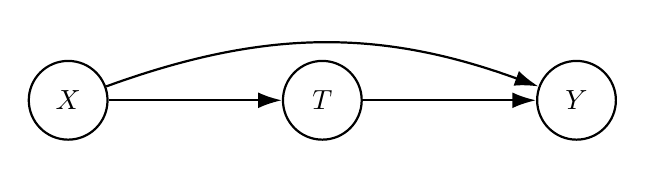
\begin{tikzpicture}[node distance=2.2cm]
        \node[dagnode] (X) {$X$};
        \node[dagnode, right=of X] (T) {$T$};
        \node[dagnode, right=of T] (Y) {$Y$};
        \draw[dagarrow] (X) -- (T);
        \draw[dagarrow] (X) to[out=20,in=160] (Y);
        \draw[dagarrow] (T) -- (Y);
    \end{tikzpicture}
    \caption{Causal structure assumed throughout. The treatment $T$ is continuous and
    possibly multidimensional, the outcome $Y$ is scalar, and the covariates $X$ affect
    both. The only back-door path $T \leftarrow X \rightarrow Y$ is blocked by conditioning
    on $X$.}
    \label{fig:dag}
\end{figure}

To turn this structure into identification of the potential outcomes
$\{Y(t) : t \in \cT\}$, we impose the standard conditions for continuous treatments, due to
\citet{imbens2000} and \citet{hirano2004}.

\begin{assumption}[Identification]
\label{as:identification}
Let $t \in \cT$ be the treatment level of interest.
\begin{enumerate}
\item[(i)] \emph{Consistency and no interference.} $Y = Y(T)$, and a unit's potential
outcomes do not depend on the treatment levels of other units.
\item[(ii)] \emph{Weak unconfoundedness.} $Y(t) \perp T \mid X$.
\item[(iii)] \emph{Positivity.} There exists $\gps_{\min} > 0$ such that
$\pf{T \mid X=x}(t) \ge \gps_{\min}$ for every $x$ with $\pf{X}(x) > 0$.
\end{enumerate}
\end{assumption}

The three parts play distinct roles. Consistency ties the potential outcomes to the observed
data, equating $Y$ with the potential outcome at the treatment actually received. Weak
unconfoundedness is the distributional counterpart of the absent common cause of $T$ and $Y$
in Figure~\ref{fig:dag}: given the covariates, the treatment carries no further information
about the potential outcome. Positivity requires the level $t$ to be reachable at every
covariate value; its lower bound $\gps_{\min}$ is what will keep the correction of
Section~\ref{sec:eif} finite. Under these conditions $Y(t)$ is identified, because weak
unconfoundedness makes the conditional density of $Y$ at $T=t$ equal to the density of $Y(t)$
at each covariate value, and averaging over the covariates recovers the interventional law.

\begin{mydef}[Interventional density]
\label{def:target}
For $t \in \cT$ and $y \in \cY$, the interventional density is
\begin{equation}
p_t(y) \;:=\; \pf{Y(t)}(y) \;=\; \pE_X\big[\eta(X)\big]
\;=\; \int_{\cX} \eta(x)\,\pf{X}(x) \dd x ,
\qquad
\eta(x) := \pf{Y \mid T=t,X=x}(y),
\label{eq:target}
\end{equation}
where $\eta(x)$ is the conditional outcome density at the point $(t,x,y)$; we suppress its
dependence on the fixed $t$ and $y$.
\end{mydef}

Two features of this estimand matter later. First, the covariate is averaged out while $t$ and
$y$ are fixed evaluation points; this asymmetry is what produces the point masses in the
influence function. Second, the only unknown is the conditional density $\eta$, since the
covariate distribution is handled by the empirical distribution of $X_1,\dots,X_n$. Its
conditioning set $(T,X)$ has dimension $d+p$ while the outcome is scalar, and it is this
imbalance that makes standard estimators inaccurate and motivates the estimator used below.

The correction of Section~\ref{sec:eif} will also involve the conditional law of the
treatment, which we introduce here.

\begin{mydef}[Generalized propensity score]
\label{def:gps}
The conditional density of the treatment given the covariates,
\begin{equation}
\gps(t \mid x) \;:=\; \pf{T \mid X=x}(t),
\label{eq:gps}
\end{equation}
is the generalized propensity score of \citet{imbens2000} and \citet{hirano2004}.
\end{mydef}

For a continuous treatment $\gps(t\mid x)$ is a density in $t \in \R^{d}$, not a probability,
and part~(iii) of Assumption~\ref{as:identification} bounds it below. It plays no role in
identification --- the estimand~\eqref{eq:target} does not mention it --- and its cost as a
nuisance is precisely what the contrastive route will save.

\subsection{The conditional density estimator}
\label{sec:setting-mcd}

By Definition~\ref{def:target}, estimating $p_t(y)$ comes down to estimating the conditional
density $\eta$ and averaging it over the covariates. Any estimator of $\eta$ may be used, and
the correction we develop later does not depend on the choice; but the choice determines the
accuracy, and classical estimators do poorly here. Their rates fall with the dimension of the
conditioning argument
\citep{stone1980,Tsybakov2009NonparametricEstimation,bashtannyk2001,hall2004}, here $d+p$, so
with several treatments and confounders this error dominates everything else.

Marginal contrastive discrimination avoids fitting any density on $\cT \times \cX$. It
replaces the conditional density by two objects that are individually easy: the univariate
marginal $\pf{Y}$, and a density ratio recovered by binary classification. On problems of
this shape the method is competitive with state-of-the-art conditional-density estimators at
lower cost; we refer to \citet{meziani2025mcd} for those comparisons. We use it with
conditioning variable $(T,X)$ and target variable $Y$. It starts from the elementary
factorization
\begin{equation}
\pf{Y \mid T=t,X=x}(y)
\;=\; \pf{Y}(y) \cdot \DensityRatio(t,x,y),
\qquad
\DensityRatio(t,x,y) := \frac{\pf{T,X,Y}(t,x,y)}{\pf{T,X}(t,x)\,\pf{Y}(y)} ,
\label{eq:reformulation}
\end{equation}
valid when $\pf{T,X}(t,x) > 0$ and $\pf{Y}(y) > 0$. The first factor is a univariate marginal;
the second is a density ratio that equals one when $Y$ is independent of $(T,X)$ and otherwise
measures their dependence. The classifier learns this ratio.

\begin{mydef}[Marginal contrast function, $\MCF(\ratio)$]
\label{def:MCF}
For a mixture ratio $\ratio \in (0,1)$,
\begin{equation}
\contrast(t,x,y)
\;=\; \frac{\ratio\,\pf{T,X,Y}(t,x,y)}
{\ratio\,\pf{T,X,Y}(t,x,y) + (1-\ratio)\,\pf{T,X}(t,x)\,\pf{Y}(y)} .
\label{eq:contrast}
\end{equation}
\end{mydef}

Definition~\ref{def:MCF} is best read as a posterior probability. Consider the experiment in
which a label $Z\in\{0,1\}$ is drawn with $\pP(Z=1)=\ratio$; when $Z=1$ one records an
observed vector $W=(T,X,Y)$, and when $Z=0$ one records $W=(T,X,\widetilde Y)$ with
$\widetilde Y \sim \pf{Y}$ drawn independently of $(T,X)$. Then $\contrast(t,x,y)$ is exactly
$\pP[Z=1 \mid W=(t,x,y)]$, so recovering the contrast function is a supervised classification
problem: tell a genuine triple from one whose outcome has been swapped for an independent
draw. In practice one builds a contrastive dataset
$\mDwz{N}=\{(W_i,Z_i)\}_{i=1}^{N}$ --- the condition $\MDC(\ratio)$ of \citet{meziani2025mcd}
--- by labelling each observed vector $Z=1$ and adjoining vectors with resampled outcomes
labelled $Z=0$.

The classifier and the density ratio encode the same information, so either recovers the
other, and hence the conditional density. This is the content of the next identity, which we
use repeatedly.

\begin{mypropo}[Reconstruction identity]
\label{prop:reconstruction}
For all $(t,x,y)$ with $\pf{T,X}(t,x) > 0$ and $\pf{Y}(y) > 0$,
\begin{equation}
\pf{Y \mid T=t,X=x}(y) \;=\; \pf{Y}(y)\,\DensityRatio(t,x,y),
\qquad
\DensityRatio(t,x,y) \;=\; \frac{1-\ratio}{\ratio}\,
\frac{\contrast(t,x,y)}{1-\contrast(t,x,y)} .
\label{eq:reconstruction}
\end{equation}
\end{mypropo}

This is Lemma~1 of \citet{meziani2025mcd}, specialized to conditioning variable $(T,X)$; we
reproduce the short proof in Appendix~\ref{app:mcd-reconstruction} for completeness. The
mixture ratio $\ratio$ is a design parameter: different values give different contrast
functions but the same density ratio, provided the value used to build $\mDwz{N}$ is the one
substituted into~\eqref{eq:reconstruction}.

A contrast estimate $\contrasthat$ and a marginal estimate $\pfhat{Y}$ then combine, through
the second identity in~\eqref{eq:reconstruction}, into an estimate of the conditional density,
\[
\widehat\eta(x) \;=\; \pfhat{Y}(y)\,\widehat{\DensityRatio}(t,x,y),
\qquad
\widehat{\DensityRatio} \;=\; \frac{1-\ratio}{\ratio}\,
\frac{\contrasthat}{1-\contrasthat} .
\]
Nothing forces $\widehat\eta$ to integrate to one in $y$; \citet{meziani2025mcd} restore this
by a rescaling step, which we adopt.

Two features of the construction return later. The negative class is built from the data by
recombination, so the classifier's training law is itself a functional of $F$; this is what
makes its influence function depart from the usual formula. And because the classifier only
compares observed vectors with recombined ones, it works on the support of the joint law rather
than the ambient space, which is why the construction stays feasible when $d+p$ is large
\citep{meziani2025mcd}.

\subsection{The plug-in estimator and its first-order bias}
\label{sec:setting-plugin}

Let $\widehat\eta$ be any estimator of the conditional density $\eta$ --- the contrastive
estimator above is one choice, but nothing in this subsection uses it. Averaging
$\widehat\eta$ over the covariates, as Definition~\ref{def:target} prescribes, gives the
plug-in estimator
\begin{equation}
\widehat p^{\,\mathrm{pi}}_t(y)
\;=\; \frac{1}{n} \sum_{i=1}^{n} \widehat\eta(X_i).
\label{eq:plugin}
\end{equation}
To see why this estimator is biased, suppose $\widehat\eta$ is fitted on a sample independent
of $X_1,\dots,X_n$, and split the error by adding and subtracting the covariate average of the
true $\eta$:
\begin{equation}
\widehat p^{\,\mathrm{pi}}_t(y) - p_t(y)
= \underbrace{\frac1n \sum_{i=1}^n \big( \eta(X_i) - p_t(y) \big)}_{\text{sampling error}}
\;+\; \underbrace{\frac1n \sum_{i=1}^n \big( \widehat\eta(X_i) - \eta(X_i) \big)}_{\text{nuisance error}} .
\label{eq:plugin-decomp}
\end{equation}
The two pieces behave in opposite ways. The sampling error averages the fixed function
$x\mapsto\eta(x)-p_t(y)$, which has mean zero because $\pE_X[\eta(X)] = p_t(y)$; it is
therefore centred and of order $n^{-1/2}$, the ordinary fluctuation of a sample mean.

The nuisance error behaves differently. Because
$\widehat\eta$ is fitted on a separate sample, we may treat it as fixed and take expectations
over $X_1,\dots,X_n$ alone. Each term then has the same expectation, so
\begin{equation}
\pE\Big[\, \widehat p^{\,\mathrm{pi}}_t(y) - p_t(y) \,\Big|\, \widehat\eta \,\Big]
= \pE_X\big[ \widehat\eta(X) - \eta(X) \big],
\label{eq:plugin-bias}
\end{equation}
the average error of the conditional-density estimate. Nothing forces this quantity to vanish:
if $\widehat\eta$ over- or under-estimates $\eta$ on average, so does the plug-in. The offset
is a property of the back-door average itself, shared by every conditional-density estimator,
not an accident of any particular $\widehat\eta$.

The right-hand side of~\eqref{eq:plugin-bias} is what the semiparametric literature calls the
first-order bias of the plug-in, and the name deserves a word of caution, since it is not the
bias of an estimator in the elementary sense. The finite-sample bias
$\pE[\widehat\theta]-\theta$ at a fixed model would vanish as the nuisance became consistent;
the quantity in~\eqref{eq:plugin-bias} is a different object, namely the leading term of the
estimation error expanded in the nuisance error $\widehat\eta-\eta$, and it is of first order
precisely because it is linear in that error. The same term recurs across the literature under
names that stress different facets of it: an obstruction to efficient estimation with an
infinite-dimensional nuisance \citep{bickel1988,robins2008}, a regularization bias inherited
from the smoothing that any flexible estimator applies \citep{chernozhukov2018}, or the plug-in
bias that the one-step correction is built to remove
\citep{vanderlaan2006tmle,kennedy2022review}. We adopt the term first-order bias for the
object~\eqref{eq:plugin-bias}.

A larger sample does not cure this bias. The nuisance error shrinks with $n$, but only at the
rate of $\|\widehat\eta-\eta\|$, and for a conditional density on a conditioning set of
dimension $d+p$ that rate is slower than $n^{-1/2}$ for any flexible estimator, as recalled in
Section~\ref{sec:setting-mcd}. On the $\sqrt n$ scale the first-order bias therefore diverges
rather than settling, so $\sqrt n\big(\widehat p^{\,\mathrm{pi}}_t(y)-p_t(y)\big)$ has no
centred limit and yields no valid confidence interval. The obstruction is not a small sample
but the sub-parametric rate of conditional-density estimation in high dimension, which no
sample size and no choice of estimator overcomes.

For the interventional density the consequence is more damaging than for a mean. The density
is estimated pointwise in $y$, so the first-order bias is not one mislocated number but a
systematic distortion of the whole curve $y\mapsto\widehat p_t(y)$. The very quantities that
motivate estimating a density --- tail probabilities, dispersion, the chance of exceeding a
threshold --- are functionals of this curve, and each inherits the distortion. Correcting the
first-order bias is thus a prerequisite for the inferences the interventional density is meant
to support, not a cosmetic refinement.

The remedy is to make the nuisance enter only at second order. A second-order term is
quadratic in $\widehat\eta-\eta$, of order $\|\widehat\eta-\eta\|^2$, which is $o(n^{-1/2})$ as
soon as the nuisance converges faster than $n^{-1/4}$ --- a requirement far weaker than the
parametric rate. The device that achieves this is the one-step correction, to which we now
turn.

\section{First-order correction}
\label{sec:eif}

The plug-in of Section~\ref{sec:setting-plugin} carries the first-order
bias~\eqref{eq:plugin-bias}, and the previous section argued that removing it is necessary
before any inference. The one-step correction does so by adding to the plug-in the empirical
average of an influence function, chosen so that the first-order term cancels and the nuisance
enters only at second order. To build it we need the influence function of $p_t(y)$. We first
recall the von Mises expansion that defines it, then compute it, and then confront the
difficulty it raises: the correction it produces is valid, but it reintroduces the generalized
propensity score. That difficulty is what motivates Section~\ref{sec:mcd-correction}.

\subsection{Von Mises expansion}
\label{sec:eif-vm}

View the target as a functional $\psi(F) = p_t(y)$ of the data law. To probe its sensitivity
to the data, perturb $F$ towards a point mass at $w \in \cW$,
\begin{equation}
F_\varepsilon \;=\; (1-\varepsilon)F + \varepsilon\,\delta_w ,
\qquad \varepsilon \in [0,1),
\label{eq:perturbation}
\end{equation}
and differentiate the target along this path. The derivative is the influence function, in the
sense of \citet{hampel1974} and the semiparametric development of \citet{bickel1993}.

\begin{mydef}[Influence function]
\label{def:if}
The influence function of $\psi$ at $F$ in the direction $\delta_w$ is
\[
\IF(w;\psi,F) \;:=\;
\frac{\partial}{\partial \varepsilon} \psi(F_\varepsilon)\Big|_{\varepsilon=0} .
\]
\end{mydef}

Because $\varepsilon \mapsto \psi(F_\varepsilon)$ is an ordinary real-valued map, its
derivative obeys the ordinary sum, product, quotient and chain rules. We collect these rules,
in the form adapted to $\IF$, in Appendix~\ref{app:toolbox}; they are all the machinery the
computations below require. The influence function has mean zero,
$\pE_F[\IF(W;\psi,F)] = 0$, and it governs the first-order response of the target to a change
of law: for any competing law $F'$,
\begin{equation}
\psi(F') - \psi(F)
\;=\; \pE_{F'}\big[\IF(W;\psi,F)\big] + \Rem_2(F',F),
\label{eq:von-mises}
\end{equation}
with a remainder of second order in $F'-F$. This expansion is what makes bias removal
possible. Reading $F'$ as the true law and $F$ as the estimated one, the plug-in error is the
first-order term plus a second-order remainder; adding the empirical average of the estimated
influence function to the plug-in cancels that first-order term and leaves only the remainder
\citep{bickel1993,vandervaart1998,vanderlaan2006tmle,chernozhukov2018}. It remains to compute
$\IF(w;p_t(y),F)$, which is the task of the next subsection.

\subsection{The influence function of the interventional density}
\label{sec:eif-classical}

We apply Definition~\ref{def:if} to the target. Since $p_t(y)$ is an integral over $x$ of a
ratio of densities in $(t,x,y)$, differentiating it along the path~\eqref{eq:perturbation}
with the calculus of Appendix~\ref{app:toolbox} yields the following; the full derivation is in
Appendix~\ref{app:classical-derivative}.

\begin{mypropo}[Nonparametric correction]
\label{prop:eif}
Under Assumption~\ref{as:identification} and the regularity conditions of
Appendix~\ref{app:classical-regularity}, the influence function of $p_t(y)$ at $F$, evaluated
at $w = (t_w,x_w,y_w)$, is
\begin{equation}
\IF\big(w; p_t(y), F\big)
= \frac{\delta_{t_w}(t)}{\gps(t \mid x_w)}
\Big( \delta_{y_w}(y) - \eta(x_w) \Big)
+ \eta(x_w) - p_t(y),
\label{eq:eif-dirac}
\end{equation}
where $\delta_a$ denotes the Dirac measure at $a$ and $\eta(x_w)=\pf{Y\mid T=t,X=x_w}(y)$.
\end{mypropo}

The shape of~\eqref{eq:eif-dirac} is exactly the shape anticipated after
Definition~\ref{def:target}, and reading it that way explains each term rather than merely
labelling it. Because the covariate is averaged out, a contamination at $x_w$ enters the
target smoothly, and its effect is the ordinary centred comparison $\eta(x_w) - p_t(y)$
between the conditional density at the contaminating covariate and its average --- the same
term one would obtain for any smooth average. Because the treatment and outcome are read off
at fixed points, by contrast, a contamination that lands on those points has a singular
effect: it can only register through Dirac masses in $t$ and $y$, which is the first term.
The weight $1/\gps(t\mid x_w)$ on that term is the inverse generalized propensity score, and
it is there for a familiar reason --- a contamination at treatment level $t_w$ is informative
about the level $t$ only in proportion to how rarely that level occurs at $x_w$, so its
influence is inflated when $\gps(t\mid x_w)$ is small. The essential observation for what
follows is simply that $\gps$ appears at all: an object absent from the
target~\eqref{eq:target} has entered its influence function.

Two limiting cases place~\eqref{eq:eif-dirac} in the literature and confirm it. For a discrete
treatment the Dirac in $t$ becomes an indicator, the generalized propensity score becomes an
ordinary propensity score, and the expression reduces to the influence function of
\citet{kennedy2023density}. For the mean $\pE[Y(t)]$ the outcome is integrated rather than
evaluated, the Dirac in $y$ disappears, and the expression reduces to that of
\citet{kennedy2017continuous}. Our target combines a continuous treatment with a pointwise
outcome, and both singular features appear together; to our knowledge this influence function
has not been derived before in that combination. It is contribution~(C1).

The Dirac masses are not estimable, so we regularize them by kernel smoothing with bandwidths
$h_T$ and $h_Y$; the substitution and its bias are carried out in
Appendix~\ref{app:classical-kernels}. Feeding the smoothed influence function into the
one-step construction of~\eqref{eq:von-mises} gives the corrected estimator
\begin{equation}
\widehat p^{\,\mathrm{c}}_t(y)
= \frac{1}{n}\sum_{i=1}^{n}
\left[ \frac{K_{h_T}(T_i-t)}{\widehat\gps(t \mid X_i)}
\Big( K_{h_Y}(Y_i-y) - \widehat\eta(X_i) \Big)
+ \widehat\eta(X_i) \right].
\label{eq:est-classical}
\end{equation}
Smoothing enters only through the two point evaluations; the nuisances $\gps$ and $\eta$ are
left unsmoothed and may be fitted by any method. This estimator removes the first-order bias
of the plug-in, and does so robustly, in the following precise sense; the remainder is bounded
in Appendix~\ref{app:classical-remainder}.

\begin{mypropo}[Double robustness]
\label{prop:dr-classical}
Under the conditions of Appendix~\ref{app:classical-remainder}, the second-order remainder of
the estimator~\eqref{eq:est-classical} factorizes as a product of the errors of $\gps$ and
$\eta$. Consequently $\widehat p^{\,\mathrm{c}}_t(y)$ is $\sqrt{n}$-consistent whenever each
nuisance converges at rate $n^{-1/4}$, and one nuisance may converge more slowly if the other
converges faster.
\end{mypropo}

\subsection{The cost of the correction}
\label{sec:eif-cost}

The estimator~\eqref{eq:est-classical} works, but it comes at a price, and naming the price is
what motivates the rest of the paper. The correction has introduced a second nuisance, the
generalized propensity score $\gps$. For a vector treatment $\gps$ is a conditional density on
$\R^{d}$, and estimating it suffers exactly the rate degradation that made the plug-in slow to
begin with, as noted in Section~\ref{sec:setting-mcd}. The correction has therefore
reintroduced, as a second nuisance, the very kind of object the contrastive construction was
chosen to avoid. Double robustness would let one nuisance be slow if the other were fast, but
here $\gps$ and $\eta$ are both conditional densities in the treatment coordinate, and both
are slow, so the guarantee is empty in the regime that matters.

There is a way out, and it uses the property of the influence function recorded in the
introduction: the influence function is unique, but the target can be written in several
equivalent forms, and differentiating each yields a different-looking but equal expression for
the same $\IF$. So far we differentiated the target in its back-door form~\eqref{eq:target},
and that form produced $\gps$. The reconstruction identity~\eqref{eq:reconstruction} supplies
a second, contrastive, form of the same target. The next section differentiates that form
instead, and obtains an expression for the same influence function in which $\gps$ no longer
appears and $\eta$ enters only through its two contrastive factors.

\section{Correction through the contrastive factorization}
\label{sec:mcd-correction}

Section~\ref{sec:eif} produced a correct correction and then showed its cost: the influence
function of the target contains the generalized propensity score, a second high-dimensional
conditional density. This section removes that cost. We rewrite the target through the
contrastive factorization, differentiate the new form, and find that the generalized
propensity score is gone. The price is a new object, the influence function of the fitted contrast function. We build the
corrected estimator of the interventional density around this object, then devote a separate part
to computing it --- in general, and in closed form for a penalized logistic contrast --- and
close with the limiting distribution.

\subsection{The contrastive form of the correction}
\label{sec:mcd-form}

We begin with the central result of the paper, contribution~(C2): the same influence function,
recomputed from the contrastive factorization, no longer contains the generalized propensity
score. Substituting the reconstruction identity~\eqref{eq:reconstruction} into the
target~\eqref{eq:target} factorizes it into a univariate marginal and a covariate-averaged
density ratio,
\begin{equation}
p_t(y) \;=\; \pf{Y}(y)\,m(t,y),
\qquad
m(t,y) \;:=\; \pE_X\big[\DensityRatio(t,X,y)\big] .
\label{eq:factorization}
\end{equation}
Both factors are functionals of $F$, and both are estimated from the same data, so a
perturbation of $F$ moves them together. Differentiating this product with the calculus of
Appendix~\ref{app:toolbox} gives the following; the derivation is in
Appendix~\ref{app:mcd-derivation}.

\begin{mypropo}[Contrastive form]
\label{prop:if-mcd}
Under the conditions of Appendix~\ref{app:mcd}, with $\contrast$ evaluated at $(t,X,y)$ inside
the expectations,
\begin{equation}
\begin{aligned}
\IF\big(w;p_t(y),F\big)
&= \pf{Y}(y)\left\{
\DensityRatio(t,x_w,y) - m(t,y)
+ \frac{1-\ratio}{\ratio}\,
\pE_X\!\left[ \frac{\IF\big(w;\contrast,F\big)}{\big(1-\contrast\big)^{2}} \right]
\right\} \\
&\quad + m(t,y)\Big( \delta_{y_w}(y) - \pf{Y}(y) \Big).
\end{aligned}
\label{eq:if-mcd}
\end{equation}
\end{mypropo}

Each group of terms in~\eqref{eq:if-mcd} has a clear provenance, and knowing where it comes
from is what makes the formula usable. The first two terms are the ordinary centred
contribution of the covariate average, now written for the density ratio rather than the
conditional density directly. The bracketed expectation carries the influence function of the
contrast function itself, and appears because the density ratio is not observed but fitted; it
is the whole subject of Section~\ref{sec:mcd-if-classifier}. The final term is the correction
attached to the univariate marginal, and it is the only place where a point evaluation
survives: the outcome is read off at $y$ inside $\pf{Y}(y)$, and the corresponding Dirac is
regularized by $K_{h_Y}$ exactly as in Section~\ref{sec:eif-classical}. Crucially, no Dirac
appears in the treatment argument, because the contrast function is evaluated at $(t,X,y)$
through a fitted model rather than through a point mass of the data.

The generalized propensity score is absent from~\eqref{eq:if-mcd}. The conditional outcome
density is still present --- by the reconstruction identity of
Proposition~\ref{prop:reconstruction}, $\pf{Y}(y)\,\DensityRatio(t,x_w,y)$ is exactly that
density --- but it enters only through the two factors of~\eqref{eq:reformulation}, a univariate
marginal and a contrast function, neither of which is a conditional density in the treatment
coordinate. The influence function is unique, so this contrastive form and the back-door
form~\eqref{eq:eif-dirac} are two expressions of the same object; we work from the contrastive
one, in which the propensity score never appears, and build the corrected estimator around it.

\subsection{The corrected estimator of the interventional density}
\label{sec:mcd-estimator-form}

The contrastive influence function of Proposition~\ref{prop:if-mcd} is all that the one-step
construction of Section~\ref{sec:eif-vm} needs. Adding the empirical average of the estimated
influence function to the plug-in, and regularizing the one surviving Dirac by $K_{h_Y}$ as in
Section~\ref{sec:eif-classical}, gives the corrected estimator
\begin{equation}
\widehat p_t(y)
= \frac{1}{n}\sum_{i=1}^{n} \left\{
\pfhat{Y}(y)\Big[
\widehat{\DensityRatio}(t,X_i,y) - \widehat m(t,y)
+ \frac{1-\ratio}{\ratio}\,\frac{1}{n}\sum_{j=1}^{n}
\frac{\widehat{\IF}\big(W_i;\contrast(t,X_j,y)\big)}{\big(1-\contrasthat(t,X_j,y)\big)^{2}}
\Big]
+ \widehat m(t,y)\, K_{h_Y}(Y_i - y)
\right\},
\label{eq:estimator-general}
\end{equation}
with $\widehat m(t,y) = n^{-1}\sum_{j} \widehat{\DensityRatio}(t,X_j,y)$. Two properties are
already visible, and together they are the payoff of the whole contrastive route: the estimator
uses no generalized propensity score, and its only bandwidth is $h_Y$, tied to the point
evaluation of the outcome, so no smoothing is performed in the treatment coordinate.

Only one ingredient remains unspecified: $\widehat{\IF}\big(W_i;\contrast\big)$, the influence
function of the fitted contrast function. Everything else in~\eqref{eq:estimator-general} is
supplied by the contrastive estimator of Section~\ref{sec:setting-mcd} --- the marginal
$\pfhat{Y}$, the density ratio $\widehat{\DensityRatio}$, and their covariate average
$\widehat m$. That last object is not a standard model influence function, because the classifier
is trained on a sample built from the data, and computing it is the task of the next two
subsections. Once it is available the correction term collapses to a single inner product per
observation (Corollary~\ref{cor:collapse}), and the estimator takes the cheap closed
form~\eqref{eq:estimator} implemented by the algorithm.

\subsection{The influence function of the contrast estimate}
\label{sec:mcd-if-classifier}

The corrected estimator~\eqref{eq:estimator-general} hinges on the one object we deferred,
$\IF(w;\contrast,F)$, the derivative of the fitted contrast function with respect to the
data-generating law. Influence functions of trained models are not new, and it helps to say why
the standard formula does not apply here. For penalized $M$-estimators the influence function is the classical sandwich
expression, treated in modern form by \citet{avella2017}. In the machine-learning literature
\citet{kohliang2017} reintroduced influence functions as a tool for interpreting trained
predictors, and their behaviour in that setting was studied by \citet{basu2021} and
\citet{bae2022}. Every one of these formulas describes the effect of perturbing a
\emph{fixed} training distribution.

The contrastive construction breaks that assumption. The negative class of $\mDwz{N}$ is
generated from the observed data, so the law of the training sample depends on $F$ through two
of its marginals. Perturbing $F$ therefore perturbs the training distribution as well as the
evaluation distribution, and the derivative acquires terms the classical formula does not have.
To make this precise, write the two component laws of the contrastive experiment as
\begin{equation}
P_1(F) := F_{T,X,Y}, \qquad
P_0(F) := F_{T,X} \otimes F_Y ,
\label{eq:laws}
\end{equation}
and let $\pE_{P_\ratio} := \ratio\,\pE_{P_1} + (1-\ratio)\,\pE_{P_0}$ be expectation under the
mixture prescribed by $\MDC(\ratio)$. The positive law $P_1(F)$ is $F$ itself, but the negative
law $P_0(F)$ is a \emph{product} of two marginals of $F$, and a contamination of $F$ perturbs
each factor of that product separately. It is this product structure that produces the extra
channels, as the logistic case will now show explicitly.

\subsection{The penalized logistic contrast}
\label{sec:mcd-logistic}

We now specialize to a contrast estimate obtained by penalized logistic regression on a fixed
feature map. There are two reasons for this choice. It is the loss under which
\citet{meziani2025mcd} establish the Bayes optimality of the contrast function, so it is the
natural loss to correct; and it has the regularity that the derivative of the previous
subsection requires --- the training criterion is strictly convex, its minimizer solves the
first-order condition exactly, and its Hessian is invertible with an explicit lower bound on
its spectrum.

Let $\sigma(u) = (1+e^{-u})^{-1}$, let $\phi : \cW \to \R^{\ks}$ be a fixed feature map, and
set $D_\beta(w) = \sigma\big(\beta^\top \phi(w)\big)$. With
$\ell(D,z) = -z\log D - (1-z)\log(1-D)$ the logistic loss, define the penalized risk and its
minimizer
\begin{equation}
\cR_\lambda(\beta;F) := \pE_{P_\ratio}\big[\ell(D_\beta(W),Z)\big]
+ \lambda \|\beta\|_2^2 ,
\qquad
\beta_\lambda(F) := \arg\min_{\beta} \cR_\lambda(\beta;F),
\label{eq:criterion}
\end{equation}
with $\lambda \ge 0$. Write $H_\lambda := \nabla^2_\beta \cR_\lambda(\beta_\lambda;F)$ for the
Hessian at the minimizer.

\begin{assumption}[Regularity]
\label{as:smooth}
$\lambda > 0$, the feature map $\phi$ is bounded on $\cW$, and $D_{\beta_\lambda}$ is bounded
away from $0$ and $1$ on the support of $P_\ratio$.
\end{assumption}

Appendix~\ref{app:logistic-grads} shows that under Assumption~\ref{as:smooth} the
criterion~\eqref{eq:criterion} is strictly convex, so that $\beta_\lambda(F)$ exists and is
unique, and that every eigenvalue of $H_\lambda$ is at least $2\lambda$. The unpenalized case
$\lambda = 0$ remains admissible provided $\phi$ is not collinear on the support. With this
regularity in hand, we can differentiate the minimizer along the perturbation.

\begin{theorem}[Influence function of the contrast estimate]
\label{thm:channels}
Under Assumption~\ref{as:smooth}, with $\beta = \beta_\lambda(F)$ and $w = (t_w,x_w,y_w)$,
\begin{equation}
\IF\big(w;\beta_\lambda,F\big) \;=\; -\,H_\lambda^{-1}\,\score(w;\beta),
\qquad
\score \;=\; \score_1 + \score_0^{TX} + \score_0^{Y},
\label{eq:master}
\end{equation}
where, with $u_\beta$ and $v_\beta$ the gradients of the loss at labels $1$ and $0$,
\begin{equation}
\begin{aligned}
\score_1 &= \ratio\Big( u_\beta(w) - \pE_{P_1}[u_\beta] \Big), \\
\score_0^{TX} &= (1-\ratio)\Big(
\pE_{\widetilde Y \sim F_Y}\big[ v_\beta(t_w,x_w,\widetilde Y) \big]
- \pE_{P_0}[v_\beta] \Big), \\
\score_0^{Y} &= (1-\ratio)\Big(
\pE_{(T,X) \sim F_{T,X}}\big[ v_\beta(T,X,y_w) \big]
- \pE_{P_0}[v_\beta] \Big).
\end{aligned}
\label{eq:channels}
\end{equation}
\end{theorem}

The three-channel form is contribution~(C3), and it is the point of departure from the
classical sandwich formula. The proof, in Appendices~\ref{app:logistic-channels}
and~\ref{app:logistic-ift}, applies the implicit function theorem to the first-order condition
and then differentiates the mixture law channel by channel. The interpretation follows the
source of each channel. The first, $\score_1$, is the ordinary score of an $M$-estimator,
computed under the law of the observed data; it is the only channel a fixed training
distribution would produce. The other two arise entirely from the contrastive law: since
$P_0(F)$ is a product of two marginals of $F$, contaminating $F$ contaminates each factor
separately, and the derivative of the product contributes one term per factor. These two
channels are what the formulas of \citet{avella2017} and \citet{kohliang2017} lack. They also
disappear when the negative class is drawn from a distribution fixed by the analyst, as in
noise-contrastive estimation \citep{gutmann2010nce}; in that case~\eqref{eq:master} collapses
to the classical sandwich formula, as verified in Appendix~\ref{app:logistic-centering}.

For the logistic model the three channels admit a closed form. Define the three averaged
feature vectors
\begin{equation}
b_{TX}(t_w,x_w) := \pE_{\widetilde Y \sim \pf{Y}}\big[ D_\beta \phi (t_w,x_w,\widetilde Y) \big],
\quad
b_Y(y_w) := \pE_{(T,X) \sim \pf{T,X}}\big[ D_\beta \phi (T,X,y_w) \big],
\quad
b_0 := \pE_{P_0}\big[ D_\beta \phi \big].
\label{eq:b-channels}
\end{equation}

\begin{mypropo}[Closed form]
\label{prop:closed-form}
Under Assumption~\ref{as:smooth},
\begin{equation}
\score(w;\beta)
= \ratio\big( D_\beta(w) - 1 \big)\phi(w)
+ (1-\ratio)\Big( b_{TX}(t_w,x_w) + b_Y(y_w) - b_0 \Big)
+ 2\lambda\beta_\lambda .
\label{eq:S}
\end{equation}
\end{mypropo}

The derivation is in Appendix~\ref{app:logistic-centering}. One feature of~\eqref{eq:S}
deserves comment, because it is easy to get wrong in an implementation and the next lemma
exists to guard against it. The three channels produce two contrastive centring terms, but the
first-order condition of~\eqref{eq:criterion} eliminates only one of them, so a single
uncancelled term $-(1-\ratio)b_0$ survives. That this residual must be present, and not an
error, is confirmed by the mean-zero property that any influence function has.

\begin{lem}[Zero mean]
\label{lem:zero-mean}
$\pE_{W \sim F}\big[\score(W;\beta_\lambda)\big] = 0$, and hence
$\pE_{W \sim F}\big[\IF(W;\beta_\lambda,F)\big] = 0$.
\end{lem}

Appendix~\ref{app:logistic-zero-mean} proves this using the fact that when $W \sim F$ the pair
$(T,X)$ follows $F_{T,X}$ and the outcome follows $F_Y$, so each contrastive channel averages
to $b_0$ and the residual is exactly what makes the total vanish. Dropping the term
$-(1-\ratio)b_0$ would leave a nonzero mean, which no influence function can have; the lemma
therefore also serves as a numerical check on any implementation, as discussed in
Section~\ref{sec:discussion-diagnostics}.

\subsection{The estimator in closed form}
\label{sec:mcd-estimator}

With the contrast influence function of Theorem~\ref{thm:channels} in hand, we return to the
correction term left general in the estimator~\eqref{eq:estimator-general} and put it in closed
form. The contrastive form~\eqref{eq:if-mcd} needs $\IF(w;\contrast,F)$ only through an
expectation over the covariates, and Theorem~\ref{thm:channels} shows that
$\IF(w;\beta_\lambda,F)$ does not depend on the covariates. That observation collapses the
correction term to an inner product, which is what makes the estimator cheap to evaluate.

\begin{corollary}
\label{cor:collapse}
Let $a_\lambda(t,y) := \pE_X\big[ \DensityRatio(t,X,y)\,\phi(t,X,y) \big]$. Then
\begin{equation}
\frac{1-\ratio}{\ratio}\,
\pE_X\!\left[ \frac{\IF\big(w;\contrast(t,X,y),F\big)}{\big(1-\contrast(t,X,y)\big)^{2}} \right]
\;=\; a_\lambda(t,y)^\top\, \IF\big(w;\beta_\lambda,F\big).
\label{eq:collapse}
\end{equation}
\end{corollary}

Appendix~\ref{app:logistic-collapse} proves the corollary and rewrites it, using
$\xi(t,y) := H_\lambda^{-1} a_\lambda(t,y)$, as
$a_\lambda(t,y)^\top \IF(w;\beta_\lambda,F) = -\xi(t,y)^\top \score(w;\beta)$. Combining
Proposition~\ref{prop:if-mcd}, Theorem~\ref{thm:channels} and Corollary~\ref{cor:collapse}
then gives the estimator
\begin{equation}
\widehat p_t(y)
= \frac{1}{n}\sum_{i=1}^{n} \left\{
\pfhat{Y}(y)\Big[
\widehat{\DensityRatio}(t,X_i,y) - \widehat m(t,y)
- \widehat\xi(t,y)^\top \widehat\score(W_i)
\Big]
+ \widehat m(t,y)\, K_{h_Y}(Y_i - y)
\right\},
\label{eq:estimator}
\end{equation}
where again $\widehat m(t,y) = n^{-1}\sum_{j} \widehat{\DensityRatio}(t,X_j,y)$. This is the
closed form promised in Section~\ref{sec:mcd-estimator-form}: the general correction term
of~\eqref{eq:estimator-general} has become the single inner product
$\widehat\xi(t,y)^\top\widehat\score(W_i)$, costing one linear solve per evaluation point and one
inner product per observation, and the estimator it produces uses no generalized propensity score
and smooths only in the outcome coordinate.

\subsection{Computation}
\label{sec:mcd-algorithm}

Algorithm~\ref{alg:main} implements the estimator~\eqref{eq:estimator}, and its cost is kept
low by three choices. The Hessian is a single average over the contrastive dataset and is
factorized once. The reparametrization by $\xi(t,y)$ moves the linear solve from the $n$
observations to the evaluation points, which are typically far fewer, leaving one inner product
per observation. The vectors $b_{TX}$ and $b_Y$ each require an average over a marginal for
every observation; subsampling this inner average over $S$ draws reduces the cost to
$\cO(nS\ks)$, and the induced Monte Carlo error is of order $S^{-1/2}$ inside a term that is
itself averaged over the sample. Cross-fitting \citep{chernozhukov2018} is used throughout: the
contrast function and the marginal density are fitted on one fold and the correction is
evaluated on the other, with the roles exchanged and the two estimates averaged. This removes
the empirical-process conditions that would otherwise be needed and makes the conditional-bias
identity~\eqref{eq:plugin-bias} hold exactly.

\begin{algorithm}[htbp]
\caption{Corrected estimator of $p_t(y)$ with a penalized logistic contrast}
\label{alg:main}
\begin{algorithmic}[1]
\State Split the sample into folds $\mathcal{A}$ and $\mathcal{B}$; exchange the roles and average at the end.
\State On $\mathcal{A}$, build $\mDwz{N}$ satisfying $\MDC(\ratio)$ by labelling each observed vector $Z=1$ and adjoining $\kappa$ vectors with resampled outcomes labelled $Z=0$, so that $\ratio = 1/(1+\kappa)$.
\State Fit $\betahat_\lambda$ by penalized logistic regression on $\mDwz{N}$; set $\contrasthat = \sigma(\betahat_\lambda^\top \phi)$ and $\widehat{\DensityRatio} = \tfrac{1-\ratio}{\ratio}\,\contrasthat/(1-\contrasthat)$.
\State Fit $\pfhat{Y}$ on $\mathcal{A}$ and rescale $\pfhat{Y \mid T,X}$ to integrate to one.
\State Form $\widehat H_\lambda$ as the empirical Hessian on $\mDwz{N}$ and factorize it once; form $\widehat b_0$ as an average over the contrastive part of $\mDwz{N}$.
\For{each evaluation point $(t,y)$}
  \State $\widehat a_\lambda(t,y) \gets n^{-1}\sum_j \widehat{\DensityRatio}(t,X_j,y)\,\phi(t,X_j,y)$;
  \State solve $\widehat H_\lambda\, \widehat\xi(t,y) = \widehat a_\lambda(t,y)$.
\EndFor
\For{each $W_i$ in $\mathcal{B}$}
  \State compute $\widehat b_{TX}(T_i,X_i)$ and $\widehat b_Y(Y_i)$ by subsampling the corresponding marginals;
  \State assemble $\widehat \score(W_i)$ from~\eqref{eq:S}.
\EndFor
\State Return $\widehat p_t(y)$ from~\eqref{eq:estimator}.
\end{algorithmic}
\end{algorithm}

\subsection{Asymptotic distribution}
\label{sec:mcd-asymptotics}

The contrast function is estimated within the parametric family indexed by $\phi$, and that
family need not contain the true $\contrast$. It is therefore natural to state the limit first
around the best parametric approximation and then, under an extra condition, around the true
target. Let
\begin{equation}
\theta_\lambda(t,y) := \pE_X\big[ \pf{Y}(y)\,\DensityRatio_{\beta_\lambda}(t,X,y) \big],
\qquad
\DensityRatio_{\beta} := \frac{1-\ratio}{\ratio}\,\frac{D_\beta}{1-D_\beta},
\label{eq:pseudo-true}
\end{equation}
be the functional evaluated at the minimizer $\beta_\lambda$ of~\eqref{eq:criterion}; it equals
$p_t(y)$ when the model contains the contrast function. Splitting the error at
$\theta_\lambda$,
\begin{equation}
\widehat p_t(y) - p_t(y)
= \underbrace{\widehat p_t(y) - \theta_\lambda(t,y)}_{\text{estimation}}
+ \underbrace{\theta_\lambda(t,y) - p_t(y)}_{\text{approximation}} ,
\label{eq:decomposition}
\end{equation}
separates a stochastic estimation term from a deterministic approximation term, and the theorem
treats each in turn.

\begin{theorem}[Asymptotic normality]
\label{thm:asymptotics}
Under Assumption~\ref{as:smooth}, cross-fitting, and the moment conditions of
Appendix~\ref{app:asymptotics-conditions}, the estimation term of~\eqref{eq:decomposition}
satisfies
\begin{equation}
\sqrt{n}\,\big( \widehat p_t(y) - \theta_\lambda(t,y) \big)
\;\longrightarrow\; \mathcal{N}(0,V),
\qquad
V = \pf{Y}(y)^2\, a_\lambda^\top H_\lambda^{-1} \Sigma H_\lambda^{-1} a_\lambda ,
\label{eq:sandwich}
\end{equation}
with $\Sigma = \Var\big(\score(W;\beta_\lambda)\big)$. If in addition
$\|D_{\beta_\lambda} - \contrast\|_{L_2} = o(n^{-1/2})$ and $\ks_n/n \to 0$, the same statement
holds with $\theta_\lambda(t,y)$ replaced by $p_t(y)$.
\end{theorem}

The proof is in Appendix~\ref{app:asymptotics-remainder}, and its logic is exactly the payoff
of the correction: the one-step construction reduces the estimation term to a second-order
quantity in $\betahat - \beta_\lambda$, which is the precise sense in which the first-order
bias~\eqref{eq:plugin-bias} has been removed. Because the variance is available in closed
form, confidence intervals require no resampling. The approximation term is deterministic and
enters linearly, and the additional condition of the theorem asks only that it be negligible
at the parametric scale; this is the standard requirement for sieve estimators
\citep{white1982,chen2007,farrell2021}.

\section{Discussion}
\label{sec:discussion}

Having built and analyzed the corrected estimator, we now step back to say what its guarantee
is and is not, how to check it in practice, and how it sits in the surrounding literature.

\subsection{What the correction provides}
\label{sec:discussion-dr}

The two estimators of this paper differ in a way that is easy to state and worth
understanding: the classical estimator~\eqref{eq:est-classical} is doubly robust in the pair
$\big(\gps, \pf{Y \mid T,X}\big)$, whereas the contrastive estimator~\eqref{eq:estimator} is
not doubly robust. The difference is structural rather than an artefact of the derivation, and
two facts explain it.

The classical pair consists of the two legs of the identified functional, the treatment law
and the outcome law, and double robustness is the statement that an error in one leg is
harmless if the other is estimated well. The contrastive factorization~\eqref{eq:reformulation}
dismantles this arrangement: it removes the treatment leg from the formula and splits the outcome
leg into a marginal and a density ratio. What takes the place of the pair is a single fitted
object, the contrast function, and the second-order remainder of the corrected estimator is
accordingly the \emph{square} of one nuisance error, $\|\betahat - \beta_\lambda\|^2$, rather than
a product of two errors that could cancel (Theorem~\ref{thm:asymptotics} and
Appendix~\ref{app:asymptotics-dr}). No second leg remains whose good behaviour could rescue a
poor contrast fit.

The two factors are moreover not variationally independent, so one could not treat them as an
error-cancelling pair even in principle.

\begin{mypropo}[Normalization constraint]
\label{prop:normalization}
For every $y$ with $\pf{Y}(y) > 0$,
\begin{equation}
\pE_{(T,X)}\big[ \DensityRatio(T,X,y) \big] = 1 .
\label{eq:normalization}
\end{equation}
\end{mypropo}

Appendix~\ref{app:asymptotics-normalization} proves this. The constraint holds for every $y$,
so the contrast function is tied to the marginal through a continuum of identities, and the
two are not free to vary independently.

What the correction does provide is the removal of the first-order bias~\eqref{eq:plugin-bias}
--- which is present regardless of any pairing of nuisances --- together with the closed-form
variance of Theorem~\ref{thm:asymptotics} and first-order insensitivity to the estimation
error of $\beta$. The condition that replaces double robustness bears on a single object, the
approximation error of the contrast model, and the next subsection describes how to assess it.

\subsection{Diagnostics}
\label{sec:discussion-diagnostics}

Four checks are available, and their scopes differ, so it is useful to keep them apart.

The empirical mean of $\widehat\score(W_i)$ should be close to zero, by
Lemma~\ref{lem:zero-mean}. This detects implementation errors, in particular an omitted
centring term, but it holds whether or not the contrast model is correctly specified, so it
diagnoses the code and not the model.

The empirical mean of $\widehat{\DensityRatio}(T_j,X_j,y)$ should be close to one for each
$y$, by Proposition~\ref{prop:normalization}. This assesses the coherence of the fitted
contrast with the marginal and is the sample counterpart of the rescaling step of
\citet{meziani2025mcd}.

Varying the dimension of the feature map and plotting $\widehat p_t(y)$ against $\ks$ indicates
whether the approximation error has become negligible. Stabilization supports the additional
condition of Theorem~\ref{thm:asymptotics}; continued drift indicates that it is not met. When
$\gps$ happens to be available, as in simulations, the contrastive estimator~\eqref{eq:estimator}
and the classical one~\eqref{eq:est-classical} estimate the same influence function and should
agree up to sampling error; a wider gap points to an error in one of the two constructions.

Finally, since the density ratio diverges as the contrast approaches one, the fitted values
$\contrasthat$ should not concentrate near one. Such concentration signals a region where
observed and recombined vectors are nearly separable, which is the contrastive symptom of a
failure of positivity, part~(iii) of Assumption~\ref{as:identification}.

\subsection{Related work}
\label{sec:discussion-lit}

The counterfactual-density estimators of \citet{kennedy2023density},
\citet{melnychuk2023flows}, \citet{ham2024logconcave} and \citet{martinez2023stein} all assume
a treatment with finitely many levels and differ in how the density is represented. The present
work departs on the treatment argument rather than the outcome representation, and
Section~\ref{sec:eif-classical} shows that the discrete-treatment correction is the limiting
case of~\eqref{eq:eif-dirac} in which the kernel degenerates into an indicator. On the
continuous-treatment side, \citet{kennedy2017continuous} and \citet{colangelo2020} target the
mean, the case in which the outcome is integrated rather than evaluated.

The influence function of the contrast estimate connects to the literature on influence
functions of trained models \citep{avella2017,kohliang2017,basu2021,bae2022}, and departs from
it in one respect: the training distribution is itself a functional of the law of the data. The
extra channels $\score_0^{TX}$ and $\score_0^{Y}$ of Theorem~\ref{thm:channels} are the
consequence, and they vanish when the negative class is drawn from a fixed distribution, as in
noise-contrastive estimation \citep{gutmann2010nce}.

\section{Conclusion}
\label{sec:conclusion}

The interventional density of a scalar outcome under a continuous, multidimensional treatment
is the covariate average of a conditional density whose conditioning set contains the treatment
and every confounder. Marginal contrastive discrimination estimates that conditional density in
a way adapted to the asymmetry between a high-dimensional conditioning set and a scalar outcome,
but the resulting plug-in inherits a first-order bias equal to the covariate average of the
nuisance error.

We derived the influence function of the target. It carries two point evaluations, one in the
treatment and one in the outcome, both regularized by kernel smoothing, and it involves the
generalized propensity score, a conditional density in the treatment coordinate. Re-expressing
the same correction through the contrastive factorization removes both nuisances from the
formula and replaces them by the influence function of the fitted contrast function, which we
computed in closed form for a penalized logistic model. Because the contrastive sample is
generated from the observed data, that influence function has three score channels rather than
one, and the two additional channels do not cancel.

The resulting estimator is asymptotically normal with a variance available in closed form, uses
no generalized propensity score, and performs no smoothing in the treatment coordinate. It is
not doubly robust, and the condition that replaces double robustness bears on the approximation
error of the contrast model alone.

\bibliographystyle{plainnat}
\bibliography{references}

\clearpage
\appendix

\section*{Appendix}
\addcontentsline{toc}{section}{Appendix}

The appendix collects all derivations, and each is written to be self-contained.
Appendix~\ref{app:toolbox} states the rules of the perturbation calculus used throughout.
Appendix~\ref{app:classical} derives the influence function of the interventional density and
the remainder of the associated estimator, proving Propositions~\ref{prop:eif}
and~\ref{prop:dr-classical}. Appendix~\ref{app:mcd} derives the contrastive form of the
correction, establishing Propositions~\ref{prop:reconstruction} and~\ref{prop:if-mcd}.
Appendix~\ref{app:logistic} treats the penalized logistic contrast, proving
Theorem~\ref{thm:channels}, Proposition~\ref{prop:closed-form}, Lemma~\ref{lem:zero-mean} and
Corollary~\ref{cor:collapse}. Appendix~\ref{app:asymptotics} contains the normalization
constraint (Proposition~\ref{prop:normalization}) and the asymptotic analysis
(Theorem~\ref{thm:asymptotics}).

\section{Perturbation calculus}
\label{app:toolbox}

Throughout this appendix $F_\varepsilon = (1-\varepsilon)F + \varepsilon\,\delta_w$ is the
contamination path of~\eqref{eq:perturbation}, and $\IF$ is the influence functional of
Definition~\ref{def:if}. The single idea behind every rule below is that
$\varepsilon \mapsto \psi(F_\varepsilon)$ is a real-valued function of one real variable, so
the ordinary rules of differentiation apply to it; each lemma is one such rule, translated into
the notation of $\IF$. We use these lemmas without further comment in
Appendices~\ref{app:classical}--\ref{app:asymptotics}.

\begin{lem}[Linearity]
\label{lem:sum}
For functionals $\psi_1,\psi_2$ admitting influence functions at $F$ and constants
$a,b \in \R$,
\[
\IF\big(w; a\psi_1 + b\psi_2, F\big)
= a\,\IF(w;\psi_1,F) + b\,\IF(w;\psi_2,F).
\]
\end{lem}
\begin{proof}
The map $\varepsilon \mapsto a\psi_1(F_\varepsilon) + b\psi_2(F_\varepsilon)$ is a linear
combination of two differentiable functions, so its derivative at $\varepsilon = 0$ is the
same linear combination of the two derivatives. By Definition~\ref{def:if} those derivatives
are $\IF(w;\psi_1,F)$ and $\IF(w;\psi_2,F)$, which gives the claimed identity.
\end{proof}

\begin{lem}[Product]
\label{lem:product}
$\IF\big(w;\psi_1\psi_2,F\big)
= \psi_1(F)\,\IF(w;\psi_2,F) + \psi_2(F)\,\IF(w;\psi_1,F)$.
\end{lem}
\begin{proof}
Set $\varphi(\varepsilon) = \psi_1(F_\varepsilon)$ and
$\chi(\varepsilon) = \psi_2(F_\varepsilon)$. The ordinary product rule gives
$(\varphi\chi)'(0) = \varphi(0)\chi'(0) + \chi(0)\varphi'(0)$. Evaluating the four factors at
$\varepsilon = 0$ using Definition~\ref{def:if}, we have $\varphi(0) = \psi_1(F)$,
$\chi(0) = \psi_2(F)$, $\varphi'(0) = \IF(w;\psi_1,F)$ and $\chi'(0) = \IF(w;\psi_2,F)$.
Substituting yields
$\psi_1(F)\,\IF(w;\psi_2,F) + \psi_2(F)\,\IF(w;\psi_1,F)$, as claimed.
\end{proof}

\begin{lem}[Quotient]
\label{lem:quotient}
If $\psi_2(F) \neq 0$,
\[
\IF\!\left(w;\frac{\psi_1}{\psi_2},F\right)
= \frac{\IF(w;\psi_1,F)}{\psi_2(F)}
- \frac{\psi_1(F)}{\psi_2(F)^2}\,\IF(w;\psi_2,F).
\]
\end{lem}
\begin{proof}
With $\varphi,\chi$ as in the previous proof and $\chi(0) = \psi_2(F) \neq 0$, the ordinary
quotient rule gives $(\varphi/\chi)'(0) = \{\varphi'(0)\chi(0) - \varphi(0)\chi'(0)\}/\chi(0)^2$.
Substituting the values of $\varphi(0),\chi(0),\varphi'(0),\chi'(0)$ from Definition~\ref{def:if}
and separating the two fractions gives the stated expression.
\end{proof}

\begin{lem}[Chain rule]
\label{lem:chain}
For $h : \R \to \R$ differentiable,
$\IF\big(w;h \circ \psi,F\big) = h'\big(\psi(F)\big)\,\IF(w;\psi,F)$.
\end{lem}
\begin{proof}
With $\chi(\varepsilon) = \psi(F_\varepsilon)$, the ordinary chain rule gives
$(h\circ\chi)'(0) = h'(\chi(0))\chi'(0)$. Since $\chi(0) = \psi(F)$ and
$\chi'(0) = \IF(w;\psi,F)$, this is $h'(\psi(F))\,\IF(w;\psi,F)$.
\end{proof}

\begin{lem}[Odds transformation]
\label{lem:odds}
Let $\psi$ take values in $(0,1)$ and $h(u) = u/(1-u)$. Then
\[
\IF\big(w;h(\psi),F\big) = \frac{\IF(w;\psi,F)}{\big(1-\psi(F)\big)^2} .
\]
In particular, since $\DensityRatio = \frac{1-\ratio}{\ratio}\, h(\contrast)$ with $\ratio$
constant,
\begin{equation}
\IF\big(w;\DensityRatio,F\big)
= \frac{1-\ratio}{\ratio}\,
\frac{\IF\big(w;\contrast,F\big)}{\big(1-\contrast\big)^{2}} .
\label{eq:app-if-R}
\end{equation}
\end{lem}
\begin{proof}
Write $h(\psi) = \psi_1/\psi_2$ with $\psi_1 = \psi$ and $\psi_2 = 1-\psi$. By
Lemma~\ref{lem:sum}, $\IF(w;1-\psi,F) = -\IF(w;\psi,F)$. Applying Lemma~\ref{lem:quotient} and
substituting this,
\[
\IF\big(w;h(\psi),F\big)
= \frac{\IF(w;\psi,F)}{1-\psi(F)}
+ \frac{\psi(F)}{(1-\psi(F))^2}\,\IF(w;\psi,F)
= \IF(w;\psi,F)\,\frac{(1-\psi(F)) + \psi(F)}{(1-\psi(F))^2},
\]
and the numerator equals $1$, which gives the first display. For the second, apply
Lemma~\ref{lem:sum} with the constant $\frac{1-\ratio}{\ratio}$ (whose influence function is
zero, being law-independent) to $\DensityRatio = \frac{1-\ratio}{\ratio} h(\contrast)$ and
substitute $\psi = \contrast$ into the first display; this is exactly~\eqref{eq:app-if-R}.
\end{proof}

\begin{lem}[Expectation of a law-dependent integrand]
\label{lem:if-expectation}
Let $h(\cdot\,;F)$ depend on $F$ both through the law of the integration variable and through
its functional form. Then
\begin{equation}
\IF\big(w; \pE_F[h(W;F)], F\big)
= h(w;F) - \pE_F\big[h(W;F)\big]
+ \pE_F\big[ \IF(w;h(\cdot\,;F),F) \big].
\label{eq:app-if-expectation}
\end{equation}
\end{lem}
\begin{proof}
By the definition of $F_\varepsilon$ as a mixture, expectation under $F_\varepsilon$ splits as
\[
\pE_{F_\varepsilon}\big[h(W;F_\varepsilon)\big]
= (1-\varepsilon)\,\pE_F\big[h(W;F_\varepsilon)\big]
+ \varepsilon\,h(w;F_\varepsilon).
\]
Differentiate at $\varepsilon = 0$, term by term. In the first summand the product rule gives
two pieces: differentiating the factor $(1-\varepsilon)$ contributes $-\pE_F[h(W;F)]$, and
differentiating the integrand contributes
$\pE_F[\partial_\varepsilon h(W;F_\varepsilon)|_{0}] = \pE_F[\IF(w;h(\cdot\,;F),F)]$, the
interchange of derivative and expectation being licensed by the regularity assumed where the
lemma is invoked. In the second summand, the factor $\varepsilon$ multiplies the derivative of
$h(w;F_\varepsilon)$, which therefore drops out at $\varepsilon = 0$, while the derivative of
$\varepsilon$ times $h(w;F_\varepsilon)$ contributes $h(w;F)$. Summing the three surviving
pieces gives~\eqref{eq:app-if-expectation}.
\end{proof}

The third term of~\eqref{eq:app-if-expectation} is what makes this lemma more than the standard
formula for the influence function of an expectation: it accounts for the dependence of the
integrand on the law, and is present precisely when the integrand is itself estimated, as the
density ratio is in Section~\ref{sec:mcd-correction}.

\section{The nonparametric correction}
\label{app:classical}

This appendix proves the results of Section~\ref{sec:eif}. Appendix~\ref{app:classical-regularity}
states the regularity conditions; Appendix~\ref{app:classical-derivative} derives the influence
function of Proposition~\ref{prop:eif}; Appendix~\ref{app:classical-kernels} regularizes its
point masses and produces the estimator~\eqref{eq:est-classical}; and
Appendix~\ref{app:classical-remainder} bounds the remainder, proving
Proposition~\ref{prop:dr-classical}.

\subsection{Regularity conditions}
\label{app:classical-regularity}

Proposition~\ref{prop:eif} holds under Assumption~\ref{as:identification} together with the
following conditions, which are those of \citet{kennedy2017continuous} and
\citet{kennedy2023density} adapted to the present target. The joint density $\pf{T,X,Y}$ is
bounded and twice continuously differentiable in $(t,y)$ in a neighbourhood of the evaluation
point; the map $y \mapsto \pf{Y}(y)$ is twice continuously differentiable at $y$; and the
kernels $K_T,K_Y$ are symmetric, of second order, with compact support. The bandwidths satisfy
$h_T,h_Y \to 0$, $n h_T^{d} h_Y \to \infty$, and the undersmoothing conditions
$\sqrt{n h_T^d h_Y}\,(h_T^2 + h_Y^2) \to 0$. The smoothness in $(t,y)$ is what allows the point
masses to be replaced by kernels with a controlled bias in
Appendix~\ref{app:classical-kernels}; the undersmoothing conditions make that bias negligible
on the $\sqrt n$ scale.

\subsection{Derivation of the influence function}
\label{app:classical-derivative}

We prove Proposition~\ref{prop:eif}. Write $f_\varepsilon$ for the density of $F_\varepsilon$
and express the target along the contamination path as
\[
p_t(y)(F_\varepsilon)
= \int_{\cX} \frac{f_\varepsilon(t,x,y)\,f_\varepsilon(x)}{f_\varepsilon(t,x)} \dd x .
\]
Because the contamination path is a mixture, $\varepsilon \mapsto f_\varepsilon$ is affine, and
each density derivative at $\varepsilon = 0$ is the difference between the corresponding point
mass and the density:
\begin{equation}
\begin{aligned}
\partial_\varepsilon f_\varepsilon(t,x,y)\big|_{0} &= \Delta(t,x,y) - \pf{T,X,Y}(t,x,y),\\
\partial_\varepsilon f_\varepsilon(x)\big|_{0} &= \Delta(x) - \pf{X}(x),\\
\partial_\varepsilon f_\varepsilon(t,x)\big|_{0} &= \Delta(t,x) - \pf{T,X}(t,x),
\end{aligned}
\label{eq:app-density-derivs}
\end{equation}
where $\Delta(t,x,y) := \delta_{t_w}(t)\,\delta_{x_w}(x)\,\delta_{y_w}(y)$ and analogously for
the marginals. Writing the integrand as $AB/C$ with $A = f_\varepsilon(t,x,y)$,
$B = f_\varepsilon(x)$ and $C = f_\varepsilon(t,x)$, ordinary calculus gives
\[
\partial_\varepsilon\!\left( \frac{AB}{C} \right)
= \frac{\dot A B}{C} + \frac{A \dot B}{C} - \frac{AB\dot C}{C^2}.
\]
Substituting~\eqref{eq:app-density-derivs} at $\varepsilon = 0$ and factoring the common
quantity $\pf{T,X,Y}(t,x,y)\pf{X}(x)/\pf{T,X}(t,x)$ out of the bracket,
\begin{equation}
\partial_\varepsilon\, p_t(y)(F_\varepsilon)\big|_{0}
= \int_{\cX} \frac{\pf{T,X,Y}(t,x,y)\,\pf{X}(x)}{\pf{T,X}(t,x)}
\left[
\frac{\Delta(t,x,y)}{\pf{T,X,Y}(t,x,y)}
+ \frac{\Delta(x)}{\pf{X}(x)}
- \frac{\Delta(t,x)}{\pf{T,X}(t,x)}
- 1
\right] \dd x ,
\label{eq:app-deriv-general}
\end{equation}
the constant $-1$ collecting the three density terms $-1-1+1$ of the three derivatives. We now
evaluate the four contributions in turn.

The term in $\Delta(x)$ contains a point mass only in the integration variable $x$, so the
integral collapses at $x = x_w$:
\[
\int_{\cX} \frac{\pf{T,X,Y}(t,x,y)}{\pf{T,X}(t,x)}\,\delta_{x_w}(x)\dd x
= \frac{\pf{T,X,Y}(t,x_w,y)}{\pf{T,X}(t,x_w)}
= \pf{Y \mid T=t,X=x_w}(y) = \eta(x_w),
\]
the integrand being continuous at $x_w$ by Appendix~\ref{app:classical-regularity}.

The term in $\Delta(t,x,y)$ carries point masses in $t$ and $y$, which are \emph{not}
integration variables and therefore remain as Dirac factors; only $\delta_{x_w}(x)$ is
integrated. Using $\gps(t \mid x) = \pf{T,X}(t,x)/\pf{X}(x)$,
\[
\int_{\cX} \frac{\pf{X}(x)}{\pf{T,X}(t,x)}\,
\delta_{t_w}(t)\delta_{x_w}(x)\delta_{y_w}(y)\dd x
= \delta_{t_w}(t)\,\delta_{y_w}(y)\,\frac{\pf{X}(x_w)}{\pf{T,X}(t,x_w)}
= \frac{\delta_{t_w}(t)\,\delta_{y_w}(y)}{\gps(t \mid x_w)} .
\]

The term in $\Delta(t,x)$ carries a point mass in $t$ only, and integrating out $\delta_{x_w}(x)$
gives, again using the definition of $\gps$,
\[
-\int_{\cX} \frac{\pf{T,X,Y}(t,x,y)\,\pf{X}(x)}{\pf{T,X}(t,x)^2}\,
\delta_{t_w}(t)\delta_{x_w}(x)\dd x
= -\,\delta_{t_w}(t)\,\frac{\pf{T,X,Y}(t,x_w,y)}{\pf{T,X}(t,x_w)}\,\frac{\pf{X}(x_w)}{\pf{T,X}(t,x_w)}\cdot\frac{\pf{T,X}(t,x_w)}{\pf{X}(x_w)}
\]
which simplifies to
$-\,\delta_{t_w}(t)\,\eta(x_w)/\gps(t \mid x_w)$.

The constant term $-1$ integrates against the factored density to $-\pE_X[\eta(X)] = -p_t(y)$
by Definition~\ref{def:target}.

Collecting the four contributions,
\[
\partial_\varepsilon\, p_t(y)(F_\varepsilon)\big|_{0}
= \frac{\delta_{t_w}(t)\,\delta_{y_w}(y)}{\gps(t \mid x_w)}
- \frac{\delta_{t_w}(t)\,\eta(x_w)}{\gps(t \mid x_w)}
+ \eta(x_w) - p_t(y),
\]
and factoring $\delta_{t_w}(t)/\gps(t\mid x_w)$ out of the first two terms yields
\[
\IF\big(w;p_t(y),F\big)
= \frac{\delta_{t_w}(t)}{\gps(t \mid x_w)}\Big(\delta_{y_w}(y) - \eta(x_w)\Big)
+ \eta(x_w) - p_t(y),
\]
which is exactly~\eqref{eq:eif-dirac}, the claim of Proposition~\ref{prop:eif}. \hfill$\square$

\subsection{Regularization of the point evaluations}
\label{app:classical-kernels}

Expression~\eqref{eq:eif-dirac} is exact but not computable, because it contains Dirac masses
in $t$ and $y$. We regularize each by a kernel. Let $K_T : \R^{d} \to \R_+$ and
$K_Y : \R \to \R_+$ be symmetric second-order kernels integrating to one, and for bandwidths
$h_T, h_Y > 0$ set
\begin{equation}
K_{h_T}(u) = h_T^{-d} K_T(u/h_T), \qquad
K_{h_Y}(v) = h_Y^{-1} K_Y(v/h_Y).
\label{eq:kernels}
\end{equation}
Substituting $\delta_{t_w}(t) \rightsquigarrow K_{h_T}(t_w - t)$ and
$\delta_{y_w}(y) \rightsquigarrow K_{h_Y}(y_w - y)$ in~\eqref{eq:eif-dirac}, and leaving the
nuisances unchanged, gives the smoothed influence function
\begin{equation}
\IF_{h}\big(w;p_t(y),F\big)
= \frac{K_{h_T}(t_w-t)}{\gps(t \mid x_w)}
\Big( K_{h_Y}(y_w-y) - \pf{Y \mid T=t,X=x_w}(y) \Big)
+ \pf{Y \mid T=t,X=x_w}(y) - p_t(y),
\label{eq:app-if-smoothed}
\end{equation}
whose empirical average, added to the plug-in and with the nuisances replaced by their
estimates, is exactly the corrected estimator~\eqref{eq:est-classical}. Under the smoothness
and undersmoothing conditions of Appendix~\ref{app:classical-regularity}, a second-order Taylor
expansion of the smoothed functional around $(t,y)$ gives
$\pE\big[\IF_h(W;p_t(y),F)\big] = \cO(h_T^2 + h_Y^2)$, so the substitution introduces a
deterministic bias of that order, which the undersmoothing conditions render negligible on the
$\sqrt n$ scale.

Two special cases recover known influence functions, and reproducing them checks the
derivation. If $T$ takes finitely many values, the point mass $\delta_{t_w}(t)$ is the
indicator $\Indi(t_w = t)$, no smoothing is needed in the treatment argument, and
$\gps(t \mid x)$ is the ordinary propensity score; \eqref{eq:app-if-smoothed} then reduces to
the influence function of \citet{kennedy2023density}. If the target is $\pE[Y(t)]$, the outcome
is integrated rather than evaluated: the derivation carries an extra factor $y$ and an extra
integral in $y$, the point mass $\delta_{y_w}(y)$ is replaced by $y_w$, and
\eqref{eq:app-if-smoothed} reduces to the influence function of \citet{kennedy2017continuous}.

\subsection{Second-order remainder}
\label{app:classical-remainder}

We prove Proposition~\ref{prop:dr-classical}. Let $\widehat\gps$ and $\pfhat{Y \mid T,X}$ be
nuisance estimates fitted on an independent fold, and write $\eta(x) := \pf{Y \mid T=t,X=x}(y)$
and $\widehat\eta(x) := \pfhat{Y \mid T=t,X=x}(y)$. Take expectations in the corrected
estimator~\eqref{eq:est-classical} conditionally on the fitting fold. By the mean-zero and
first-order-cancellation properties of the one-step correction, the terms linear in each
nuisance error vanish, and what remains is the cross term
\begin{equation}
\Rem_2
= \pE\!\left[
\left( \frac{K_{h_T}(T-t)}{\widehat\gps(t \mid X)}
- \frac{K_{h_T}(T-t)}{\gps(t \mid X)} \right)
\Big( \eta(X) - \widehat\eta(X) \Big)
\right].
\label{eq:app-remainder}
\end{equation}
This is a product of the two nuisance errors: the first factor is the error in the inverse
propensity weight and the second is the error in the conditional density. Applying the
Cauchy--Schwarz inequality and bounding $\widehat\gps^{-1}$ and $\gps^{-1}$ using the lower
bound $\gps_{\min}$ of Assumption~\ref{as:identification}(iii) and the boundedness of $K_{h_T}$,
\[
|\Rem_2| \;\lesssim\; \big\| \widehat\gps - \gps \big\|_{L_2}\,
\big\| \widehat\eta - \eta \big\|_{L_2} .
\]
The remainder is therefore controlled by the product of the two $L_2$ errors. It is
$o(n^{-1/2})$ whenever each error is $o(n^{-1/4})$, and one error may be larger if the other is
correspondingly smaller, so that the product still vanishes faster than $n^{-1/2}$; this is
exactly the double robustness asserted in Proposition~\ref{prop:dr-classical}. \hfill$\square$

\section{The contrastive correction}
\label{app:mcd}

This appendix proves the results of Section~\ref{sec:mcd-form}. We first prove the
reconstruction identity, then differentiate the contrastive factorization to obtain
Proposition~\ref{prop:if-mcd}.

\subsection{Proof of Proposition~\ref{prop:reconstruction}}
\label{app:mcd-reconstruction}

From Definition~\ref{def:MCF}, the odds of the contrast function are the ratio of its two
mixture components,
\[
\frac{\contrast}{1-\contrast}
= \frac{\ratio\,\pf{T,X,Y}(t,x,y)}{(1-\ratio)\,\pf{T,X}(t,x)\,\pf{Y}(y)}
= \frac{\ratio}{1-\ratio}\,\frac{\pf{Y \mid T=t,X=x}(y)}{\pf{Y}(y)} ,
\]
where the second equality uses the factorization
$\pf{T,X,Y}(t,x,y) = \pf{T,X}(t,x)\,\pf{Y \mid T=t,X=x}(y)$ to cancel $\pf{T,X}(t,x)$.
Multiplying both sides by $(1-\ratio)/\ratio$ isolates
$\frac{1-\ratio}{\ratio}\,\contrast/(1-\contrast) = \pf{Y \mid T=t,X=x}(y)/\pf{Y}(y)$, and by
the definition of $\DensityRatio$ in~\eqref{eq:reformulation} the left-hand side is
$\DensityRatio(t,x,y)$. Rearranging gives both
$\DensityRatio = \frac{1-\ratio}{\ratio}\,\contrast/(1-\contrast)$ and
$\pf{Y \mid T=t,X=x}(y) = \pf{Y}(y)\,\DensityRatio$, which are the two identities
of~\eqref{eq:reconstruction}. \hfill$\square$

\subsection{Proof of Proposition~\ref{prop:if-mcd}}
\label{app:mcd-derivation}

We differentiate the contrastive factorization~\eqref{eq:factorization},
$p_t(y) = \pf{Y}(y)\,m(t,y)$. By the product rule, Lemma~\ref{lem:product},
\begin{equation}
\IF\big(w;p_t(y),F\big)
= \pf{Y}(y)\,\IF\big(w;m(t,y),F\big)
+ m(t,y)\,\IF\big(w;\pf{Y}(y),F\big).
\label{eq:app-product}
\end{equation}
We compute the two influence functions on the right in turn.

For the marginal factor, $\pf{Y}(y)$ depends on $F$ only through the marginal law of the
outcome, evaluated at the fixed point $y$. This is the univariate special case of the
computation in Appendix~\ref{app:classical-derivative}: differentiating a marginal density at a
fixed point along the contamination path returns the difference between a point mass and the
density,
\begin{equation}
\IF\big(w;\pf{Y}(y),F\big) = \delta_{y_w}(y) - \pf{Y}(y),
\label{eq:app-if-fY}
\end{equation}
which is regularized by $\delta_{y_w}(y) \rightsquigarrow K_{h_Y}(y_w - y)$ as in
Appendix~\ref{app:classical-kernels}.

For the covariate-averaged factor $m(t,y) = \pE_X[\DensityRatio(t,X,y)]$, the integrand
$\DensityRatio(t,X,y;F)$ depends on $F$ both through the law of $X$ and through its own
functional form, since the density ratio is itself a functional of $F$. Lemma~\ref{lem:if-expectation}
is written for exactly this situation, and gives
\begin{equation}
\IF\big(w;m(t,y),F\big)
= \DensityRatio(t,x_w,y) - m(t,y)
+ \pE_X\big[ \IF(w;\DensityRatio(t,X,y),F) \big].
\label{eq:app-if-m}
\end{equation}
The third term is present precisely because the density ratio is fitted rather than known; it
is the term that will carry the influence function of the classifier. Substituting the odds
rule~\eqref{eq:app-if-R} of Lemma~\ref{lem:odds} for $\IF(w;\DensityRatio,F)$ inside that
expectation turns it into
$\frac{1-\ratio}{\ratio}\,\pE_X[\IF(w;\contrast,F)/(1-\contrast)^2]$.

Finally, substitute the marginal influence function~\eqref{eq:app-if-fY} and the covariate
influence function~\eqref{eq:app-if-m}, with the odds rule applied, into the
product~\eqref{eq:app-product}. Collecting the terms of $\pf{Y}(y)\,\IF(w;m(t,y),F)$ inside a
brace and keeping the marginal term separate reproduces exactly~\eqref{eq:if-mcd}, the claim of
Proposition~\ref{prop:if-mcd}. \hfill$\square$

\section{The penalized logistic contrast}
\label{app:logistic}

This appendix proves the results of Sections~\ref{sec:mcd-logistic}
and~\ref{sec:mcd-estimator}. Appendix~\ref{app:logistic-grads} records the gradients, the
Hessian and the convexity that underlie Assumption~\ref{as:smooth}.
Appendix~\ref{app:logistic-channels} differentiates the two component laws.
Appendix~\ref{app:logistic-ift} assembles these into Theorem~\ref{thm:channels}.
Appendices~\ref{app:logistic-centering} and~\ref{app:logistic-zero-mean} prove the closed form
(Proposition~\ref{prop:closed-form}) and the zero-mean property (Lemma~\ref{lem:zero-mean}), and
Appendix~\ref{app:logistic-collapse} proves Corollary~\ref{cor:collapse}. Throughout,
$\beta = \beta_\lambda(F)$, $D := D_\beta$, $\phi := \phi(t,x,y)$, and all expectations are
taken at $F$.

\subsection{Gradients, Hessian and convexity}
\label{app:logistic-grads}

Differentiating the logistic loss in its first argument,
\begin{equation}
\frac{\partial \ell}{\partial D}(D,z)
= -\frac{z}{D} + \frac{1-z}{1-D}
= \frac{D-z}{D(1-D)} .
\label{eq:app-dl}
\end{equation}
Differentiating the model in $\beta$, with $\sigma' = \sigma(1-\sigma)$,
\begin{equation}
\nabla_\beta D_\beta = D(1-D)\,\phi .
\label{eq:app-grad-D}
\end{equation}
Composing the two by the chain rule, the factor $D(1-D)$ cancels and the loss gradient
simplifies to
\begin{equation}
\nabla_\beta \ell(D_\beta,z) = (D-z)\,\phi ,
\qquad\text{so}\qquad
u_\beta = (D-1)\phi, \quad v_\beta = D\phi ,
\label{eq:app-uv}
\end{equation}
where $u_\beta$ and $v_\beta$ are the gradients at labels $z=1$ and $z=0$. Differentiating once
more and using~\eqref{eq:app-grad-D}, both labels give the same second derivative
$\nabla_\beta u_\beta = \nabla_\beta v_\beta = D(1-D)\phi\phi^\top$, so the Hessian of the
penalized risk is
\begin{equation}
H_\lambda
= \pE_{P_\ratio}\big[ D(1-D)\,\phi\phi^\top \big] + 2\lambda I_{\ks} .
\label{eq:app-hessian}
\end{equation}
For any $s \in \R^{\ks}$,
\[
s^\top H_\lambda s
= \pE_{P_\ratio}\big[ D(1-D)(s^\top\phi)^2 \big] + 2\lambda\|s\|^2
\;\ge\; 2\lambda\|s\|^2 ,
\]
since $D(1-D) > 0$ makes the first term nonnegative. Hence $H_\lambda$ is positive definite with
every eigenvalue at least $2\lambda$, the criterion~\eqref{eq:criterion} is strictly convex, and
$\beta_\lambda(F)$ exists, is unique and is interior. When $\lambda = 0$ the same computation
gives positive definiteness provided $\pE_{P_\ratio}[(s^\top\phi)^2] > 0$ for every $s \neq 0$,
i.e.\ provided $\phi$ is not collinear on the support. The first-order condition
$\nabla_\beta \cR_\lambda = 0$ reads, using~\eqref{eq:app-uv},
\begin{equation}
G_\lambda(\beta;F)
:= \ratio\,\pE_{P_1}[u_\beta] + (1-\ratio)\,\pE_{P_0}[v_\beta] + 2\lambda\beta = 0 .
\label{eq:app-foc}
\end{equation}

\subsection{Perturbation of the two component laws}
\label{app:logistic-channels}

We differentiate each component of the mixture $P_\ratio$ along the contamination path,
treating $\beta$ as fixed; the dependence of $\beta$ on $F$ is restored in
Appendix~\ref{app:logistic-ift}.

The positive law is the observed law, $P_1(F_\varepsilon) = F_\varepsilon$, so
$\pE_{F_\varepsilon}[u] = (1-\varepsilon)\pE_F[u] + \varepsilon\,u(w)$ is affine in
$\varepsilon$, and its derivative is
\begin{equation}
\partial_\varepsilon\, \pE_{P_1(F_\varepsilon)}[u]\big|_{0}
= u(w) - \pE_{P_1}[u].
\label{eq:app-channel1}
\end{equation}

The negative law is the product $P_0(F_\varepsilon) = F_{T,X,\varepsilon} \otimes F_{Y,\varepsilon}$,
whose two factors are the contaminated marginals of $F_\varepsilon$,
\[
F_{T,X,\varepsilon} = (1-\varepsilon)F_{T,X} + \varepsilon\,\delta_{(t_w,x_w)},
\qquad
F_{Y,\varepsilon} = (1-\varepsilon)F_Y + \varepsilon\,\delta_{y_w} .
\]
Expanding the double integral $\pE_{P_0(F_\varepsilon)}[v]$ into the four terms according to
which factor carries the contamination,
\begin{equation}
\begin{aligned}
\pE_{P_0(F_\varepsilon)}[v]
&= (1-\varepsilon)^2\,\pE_{P_0}[v]
+ (1-\varepsilon)\varepsilon\,\pE_{F_{T,X}}\big[ v(T,X,y_w) \big] \\
&\quad + \varepsilon(1-\varepsilon)\,\pE_{F_Y}\big[ v(t_w,x_w,\widetilde Y) \big]
+ \varepsilon^2\, v(t_w,x_w,y_w).
\end{aligned}
\label{eq:app-p0-expanded}
\end{equation}
Differentiate at $\varepsilon = 0$. The quadratic term $\varepsilon^2 v(t_w,x_w,y_w)$ has zero
derivative; the factor $(1-\varepsilon)^2$ contributes $-2\,\pE_{P_0}[v]$; and each of the two
cross terms, being $\varepsilon(1-\varepsilon)$ times a constant, contributes that constant.
Hence
\begin{equation}
\partial_\varepsilon\, \pE_{P_0(F_\varepsilon)}[v]\big|_{0}
= \pE_{F_Y}\big[ v(t_w,x_w,\widetilde Y) \big]
+ \pE_{F_{T,X}}\big[ v(T,X,y_w) \big]
- 2\,\pE_{P_0}[v].
\label{eq:app-channel0}
\end{equation}
The coefficient $-2$ on the centring term is what splits the contrastive derivative into two
channels, one for each factor of the product measure. Equivalently, applying the product rule
of Lemma~\ref{lem:product} to the bilinear map
$(\mu,\nu) \mapsto \iint v \dd\mu \dd\nu$ produces the first bracket by differentiating
$F_{T,X,\varepsilon}$ at fixed $F_Y$ and the second by differentiating $F_{Y,\varepsilon}$ at
fixed $F_{T,X}$. The mixture ratio $\ratio$ is a design constant and contributes no derivative.

\subsection{Proof of Theorem~\ref{thm:channels}}
\label{app:logistic-ift}

By definition the perturbed minimizer $\beta_\lambda(F_\varepsilon)$ solves the first-order
condition $G_\lambda\big(\beta_\lambda(F_\varepsilon);F_\varepsilon\big) = 0$ identically in
$\varepsilon$. The left-hand side depends on $\varepsilon$ in two ways, through the parameter
$\beta_\lambda(F_\varepsilon)$ and through the law $F_\varepsilon$. Differentiating the identity
at $\varepsilon = 0$ by the implicit function theorem,
\begin{equation}
\underbrace{\nabla_\beta G_\lambda}_{=\,H_\lambda}\,
\underbrace{\partial_\varepsilon \beta_\lambda(F_\varepsilon)\big|_{0}}_{=\,\IF(w;\beta_\lambda,F)}
+ \underbrace{\partial_\varepsilon G_\lambda(\beta;F_\varepsilon)\big|_{0}}_{=:\,\score(w;\beta)}
= 0 .
\label{eq:app-ift}
\end{equation}
The first factor is $\nabla_\beta G_\lambda = H_\lambda$ by~\eqref{eq:app-hessian}, and it is
invertible by Appendix~\ref{app:logistic-grads}; solving gives
$\IF(w;\beta_\lambda,F) = -H_\lambda^{-1}\score(w;\beta)$, which is the first equation
of~\eqref{eq:master}. It remains to identify $\score = \partial_\varepsilon G_\lambda|_0$.
Since $G_\lambda(\beta;F_\varepsilon)
= \ratio\,\pE_{P_1(F_\varepsilon)}[u_\beta] + (1-\ratio)\,\pE_{P_0(F_\varepsilon)}[v_\beta]
+ 2\lambda\beta$ and the penalty $2\lambda\beta$ does not depend on $F$, applying
\eqref{eq:app-channel1} with $u = u_\beta$ to the first expectation and
\eqref{eq:app-channel0} with $v = v_\beta$ to the second gives the three summands
\[
\score
= \ratio\big(u_\beta(w) - \pE_{P_1}[u_\beta]\big)
+ (1-\ratio)\Big(\pE_{F_Y}[v_\beta(t_w,x_w,\widetilde Y)] - \pE_{P_0}[v_\beta]\Big)
+ (1-\ratio)\Big(\pE_{F_{T,X}}[v_\beta(T,X,y_w)] - \pE_{P_0}[v_\beta]\Big),
\]
which are exactly $\score_1$, $\score_0^{TX}$ and $\score_0^{Y}$ of~\eqref{eq:channels}. This
establishes both equations of~\eqref{eq:master} and hence Theorem~\ref{thm:channels}. \hfill$\square$

\subsection{Proof of Proposition~\ref{prop:closed-form}}
\label{app:logistic-centering}

We evaluate the three channels for the logistic model. By~\eqref{eq:app-uv}, $v_\beta = D\phi$,
so every centring term $\pE_{P_0}[v_\beta]$ equals $\pE_{P_0}[D\phi] = b_0$, and the two
contaminated contrastive terms are $b_{TX}(t_w,x_w)$ and $b_Y(y_w)$ of~\eqref{eq:b-channels}.
Summing the three channels of~\eqref{eq:channels} and grouping the two centring terms with the
observed centring term,
\begin{equation}
\score(w;\beta)
= \ratio\,u_\beta(w) + (1-\ratio)\big( b_{TX}(t_w,x_w) + b_Y(y_w) \big)
- \Big( \ratio\,\pE_{P_1}[u_\beta] + 2(1-\ratio)\,b_0 \Big).
\label{eq:app-S-raw}
\end{equation}
The bracketed quantity contains the unknown expectation $\pE_{P_1}[u_\beta]$, which the
first-order condition~\eqref{eq:app-foc} pins down: rearranging
$\ratio\,\pE_{P_1}[u_\beta] + (1-\ratio)b_0 + 2\lambda\beta_\lambda = 0$ gives
$\ratio\,\pE_{P_1}[u_\beta] = -2\lambda\beta_\lambda - (1-\ratio)b_0$. Substituting this into the
bracket,
\begin{equation}
-\Big( \ratio\,\pE_{P_1}[u_\beta] + 2(1-\ratio)b_0 \Big)
= 2\lambda\beta_\lambda + (1-\ratio)b_0 - 2(1-\ratio)b_0
= 2\lambda\beta_\lambda - (1-\ratio)b_0 .
\label{eq:app-resolve}
\end{equation}
The uncancelled residual $-(1-\ratio)b_0$ appears because the first-order condition supplies a
single contrastive centring term whereas the channels of Theorem~\ref{thm:channels} produce
two. Combining~\eqref{eq:app-S-raw} and~\eqref{eq:app-resolve} and writing
$u_\beta = (D-1)\phi$ from~\eqref{eq:app-uv} gives
\[
\score(w;\beta)
= \ratio\big(D_\beta(w)-1\big)\phi(w)
+ (1-\ratio)\big(b_{TX}(t_w,x_w) + b_Y(y_w) - b_0\big)
+ 2\lambda\beta_\lambda,
\]
which is exactly~\eqref{eq:S}, the claim of Proposition~\ref{prop:closed-form}. \hfill$\square$

Two limiting cases are worth recording, as they connect the formula to familiar ones. Setting
$\lambda = 0$ removes the penalty term $2\lambda\beta_\lambda$. Setting in addition the two
contrastive channels to zero --- the situation of a negative class drawn from a distribution
fixed by the analyst, so that $b_{TX}$, $b_Y$ and $b_0$ carry no dependence on $F$ --- leaves
$\score(w;\beta) = \ratio\big(D_\beta(w)-1\big)\phi(w)$, and~\eqref{eq:master} becomes
$-H_0^{-1}\big(D_\beta(w) - z_w\big)\phi(w)$, the classical influence function of logistic
regression.

\subsection{Proof of Lemma~\ref{lem:zero-mean}}
\label{app:logistic-zero-mean}

We take the expectation of the closed form~\eqref{eq:S} over $W \sim F$. The key structural
fact is that when $W = (T,X,Y)$ is drawn from $F$, its first two components jointly follow
$F_{T,X}$ and its last component follows $F_Y$ --- the same marginals that define $P_0$.

The first term is an expectation under $P_1 = F_{T,X,Y}$, so it equals
$\ratio\,\pE_{P_1}[(D-1)\phi] = \ratio\,\pE_{P_1}[u_\beta]$ by~\eqref{eq:app-uv}.

The vector $b_{TX}(T,X) = \pE_{\widetilde Y \sim F_Y}[v_\beta(T,X,\widetilde Y)]$ is a function
of $(T,X)$ alone. Averaging it over $(T,X) \sim F_{T,X}$ and using Fubini together with the
product structure of $P_0$,
\[
\pE\big[ b_{TX}(T,X) \big]
= \pE_{(T,X) \sim F_{T,X}} \pE_{\widetilde Y \sim F_Y}\big[ v_\beta(T,X,\widetilde Y) \big]
= \pE_{P_0}[v_\beta] = b_0 .
\]
Symmetrically, $b_Y(Y) = \pE_{(T,X) \sim F_{T,X}}[v_\beta(T,X,Y)]$ is a function of $Y$ alone
and, averaged over $Y \sim F_Y$, also equals $b_0$.

The vectors $b_0$ and $2\lambda\beta_\lambda$ are constants and average to themselves. Summing
the four contributions,
\[
\pE\big[ \score(W;\beta) \big]
= \ratio\,\pE_{P_1}[u_\beta] + (1-\ratio)\big( b_0 + b_0 - b_0 \big) + 2\lambda\beta_\lambda
= \ratio\,\pE_{P_1}[u_\beta] + (1-\ratio)b_0 + 2\lambda\beta_\lambda,
\]
which is exactly $G_\lambda(\beta_\lambda;F)$ and therefore vanishes by the first-order
condition~\eqref{eq:app-foc}. This proves $\pE_{W\sim F}[\score(W;\beta_\lambda)] = 0$. Since
$H_\lambda$ does not depend on $w$, taking the expectation of
$\IF(w;\beta_\lambda,F) = -H_\lambda^{-1}\score(w;\beta_\lambda)$ gives
$\pE_{W\sim F}[\IF(W;\beta_\lambda,F)] = -H_\lambda^{-1}\pE[\score] = 0$, which is the second
statement of Lemma~\ref{lem:zero-mean}. \hfill$\square$

The computation also shows what would go wrong without the residual: had the term
$-(1-\ratio)b_0$ been omitted from~\eqref{eq:S}, the contrastive contributions would have summed
to $2b_0$ instead of $b_0$, and the total mean would have been $(1-\ratio)b_0 \neq 0$, which is
impossible for an influence function.

\subsection{Proof of Corollary~\ref{cor:collapse}}
\label{app:logistic-collapse}

We collapse the correction term to an inner product. By the chain rule, Lemma~\ref{lem:chain},
applied to $\beta \mapsto D_\beta(t,x,y)$ at fixed $(t,x,y)$, together with the model
gradient~\eqref{eq:app-grad-D},
\[
\IF\big(w;\contrast(t,x,y),F\big)
= \nabla_\beta D_\beta(t,x,y)^\top \IF(w;\beta_\lambda,F)
= D(1-D)\,\phi(t,x,y)^\top\,\IF\big(w;\beta_\lambda,F\big).
\]
Divide by $(1-D)^2$, multiply by $(1-\ratio)/\ratio$, and take the expectation over the
covariates. Because $\IF(w;\beta_\lambda,F)$ does not depend on $X$, it factors out of the
expectation, and the scalar weight simplifies to the density ratio,
\[
\frac{1-\ratio}{\ratio}\,\frac{D(1-D)}{(1-D)^2}
= \frac{1-\ratio}{\ratio}\,\frac{D}{1-D}
= \DensityRatio ,
\]
by the definition of $\DensityRatio_\beta$ in~\eqref{eq:pseudo-true}. Hence
\[
\frac{1-\ratio}{\ratio}\,
\pE_X\!\left[ \frac{\IF(w;\contrast(t,X,y),F)}{(1-\contrast(t,X,y))^2} \right]
= \pE_X\big[ \DensityRatio(t,X,y)\,\phi(t,X,y) \big]^\top \IF(w;\beta_\lambda,F)
= a_\lambda(t,y)^\top \IF(w;\beta_\lambda,F),
\]
which is~\eqref{eq:collapse}, the claim of Corollary~\ref{cor:collapse}. \hfill$\square$

Substituting $\IF(w;\beta_\lambda,F) = -H_\lambda^{-1}\score(w;\beta)$ and using the symmetry of
$H_\lambda$, with $\xi(t,y) := H_\lambda^{-1}a_\lambda(t,y)$,
\[
a_\lambda(t,y)^\top \IF\big(w;\beta_\lambda,F\big)
= -\,\big( H_\lambda^{-1}a_\lambda(t,y) \big)^\top \score(w;\beta)
= -\,\xi(t,y)^\top \score(w;\beta),
\]
which is the form used in the estimator~\eqref{eq:estimator} and requires one linear solve per
evaluation point rather than one per observation.

\section{Asymptotic analysis}
\label{app:asymptotics}

This appendix proves the normalization constraint of Section~\ref{sec:discussion-dr} and the
limit theorem of Section~\ref{sec:mcd-asymptotics}. Appendix~\ref{app:asymptotics-normalization}
proves Proposition~\ref{prop:normalization}; Appendix~\ref{app:asymptotics-conditions} lists the
moment conditions; Appendix~\ref{app:asymptotics-remainder} proves Theorem~\ref{thm:asymptotics};
and Appendix~\ref{app:asymptotics-dr} explains why the remainder has no product structure.

\subsection{Proof of Proposition~\ref{prop:normalization}}
\label{app:asymptotics-normalization}

Integrating the joint density over $(t,x)$ recovers the marginal of the outcome, and factoring
through the conditional density,
\[
\pf{Y}(y)
= \iint \pf{T,X,Y}(t,x,y) \dd t \dd x
= \iint \pf{T,X}(t,x)\,\pf{Y \mid T=t,X=x}(y) \dd t \dd x .
\]
Substituting the reconstruction identity~\eqref{eq:reconstruction},
$\pf{Y \mid T=t,X=x}(y) = \pf{Y}(y)\,\DensityRatio(t,x,y)$, and taking the constant $\pf{Y}(y)$
outside the integral,
\[
\pf{Y}(y)
= \pf{Y}(y) \iint \pf{T,X}(t,x)\,\DensityRatio(t,x,y) \dd t \dd x
= \pf{Y}(y)\,\pE_{(T,X)}\big[ \DensityRatio(T,X,y) \big].
\]
Since $\pf{Y}(y) > 0$, dividing both sides by it gives
$\pE_{(T,X)}[\DensityRatio(T,X,y)] = 1$, which is~\eqref{eq:normalization}, the claim of
Proposition~\ref{prop:normalization}. \hfill$\square$

Written in terms of the contrast function, the identity reads
$\pE_{(T,X)}\big[\contrast(T,X,y)/(1-\contrast(T,X,y))\big] = \ratio/(1-\ratio)$ for every such
$y$. It holds for each $y$ separately and therefore constitutes a continuum of restrictions
linking the contrast function to the marginal density of the outcome, which is the sense in
which the two factors of the correction are not variationally independent.

\subsection{Moment conditions}
\label{app:asymptotics-conditions}

Theorem~\ref{thm:asymptotics} is stated under Assumption~\ref{as:smooth}, the conditions of
Appendix~\ref{app:classical-regularity} for the bandwidth $h_Y$, cross-fitting as described in
Section~\ref{sec:mcd-algorithm}, and the following. The matrix
$\Sigma = \Var(\score(W;\beta_\lambda))$ is finite and positive definite; the map
$\beta \mapsto \theta_\lambda(t,y;\beta)$ is twice continuously differentiable in a
neighbourhood of $\beta_\lambda$ with bounded second derivative; and
$\|\betahat - \beta_\lambda\| = o_p(n^{-1/4})$. The first condition makes the limiting variance
well defined, the second licenses the second-order expansion below, and the third makes the
quadratic remainder of that expansion negligible on the $\sqrt n$ scale.

\subsection{Proof of Theorem~\ref{thm:asymptotics}}
\label{app:asymptotics-remainder}

We treat the two terms of the decomposition~\eqref{eq:decomposition} in turn, beginning with
the estimation term. Condition on the fitting fold, so that $\betahat$ and the marginal
estimate are fixed and the average is over the evaluation fold. By construction, the
estimator~\eqref{eq:estimator} is the plug-in evaluated at $\betahat$ plus the empirical average
of the estimated influence function of $\theta_\lambda$; this is what the one-step correction
adds. The defining property of that correction is that the terms linear in
$\betahat - \beta_\lambda$ cancel between the plug-in and the influence-function average. A
second-order Taylor expansion of $\beta \mapsto \theta_\lambda(t,y;\beta)$ around
$\beta_\lambda$, with the bounded second derivative of Appendix~\ref{app:asymptotics-conditions},
therefore leaves only a quadratic remainder:
\begin{equation}
\widehat p_t(y) - \theta_\lambda(t,y)
= \frac{1}{n}\sum_{i=1}^{n} \Psi(W_i)
+ \cO_p\big( \|\betahat - \beta_\lambda\|^2 \big),
\label{eq:app-estimation}
\end{equation}
where, by Proposition~\ref{prop:if-mcd} and Corollary~\ref{cor:collapse}, the summand is the
influence function of $\theta_\lambda$,
\[
\Psi(w) = \pf{Y}(y)\Big[
\DensityRatio_{\beta_\lambda}(t,x_w,y) - \theta_\lambda(t,y)/\pf{Y}(y)
- \xi(t,y)^\top \score(w;\beta_\lambda) \Big]
+ m(t,y)\big( K_{h_Y}(y_w - y) - \pf{Y}(y) \big).
\]
The summands $\Psi(W_i)$ are independent and centred --- the score channel by
Lemma~\ref{lem:zero-mean} and the remaining terms by construction of the influence function ---
so the leading average is a centred sum of i.i.d.\ terms. The remainder
in~\eqref{eq:app-estimation} is $o_p(n^{-1/2})$ under the rate condition
$\|\betahat - \beta_\lambda\| = o_p(n^{-1/4})$ of Appendix~\ref{app:asymptotics-conditions}.
Applying the central limit theorem to the leading average gives asymptotic normality with
variance $\Var(\Psi(W))$; substituting
$\IF(\cdot;\beta_\lambda,F) = -H_\lambda^{-1}\score$ and the collapse
identity~\eqref{eq:collapse} into $\Var(\Psi(W))$ turns it into the sandwich form
$V = \pf{Y}(y)^2\,a_\lambda^\top H_\lambda^{-1}\Sigma H_\lambda^{-1}a_\lambda$
of~\eqref{eq:sandwich}. Cross-fitting justifies conditioning on the fitting fold and removes the
empirical-process condition on the estimated nuisance. This establishes the first statement of
Theorem~\ref{thm:asymptotics}.

For the second statement, consider the approximation term $\theta_\lambda(t,y) - p_t(y)$
of~\eqref{eq:decomposition}. It is deterministic and enters the decomposition linearly, and by
the definition~\eqref{eq:pseudo-true} of $\theta_\lambda$ it is bounded above, under
Assumption~\ref{as:smooth}, by a constant multiple of $\|D_{\beta_\lambda} - \contrast\|_{L_2}$.
The stated condition $\|D_{\beta_\lambda} - \contrast\|_{L_2} = o(n^{-1/2})$ therefore makes the
approximation term negligible at the parametric scale, and the condition $\ks_n/n \to 0$ controls
the variance of the $\ks$-dimensional linear solve, as is standard for sieve estimators
\citep{chen2007,farrell2021}. Under both conditions the limit of the estimation term holds with
$\theta_\lambda(t,y)$ replaced by $p_t(y)$, which is the second statement of the theorem. \hfill$\square$

\subsection{Absence of a product structure in the remainder}
\label{app:asymptotics-dr}

It is instructive to compare the remainder~\eqref{eq:app-estimation} of the contrastive route
with the remainder~\eqref{eq:app-remainder} of the nonparametric correction, because the
comparison explains the loss of double robustness discussed in Section~\ref{sec:discussion-dr}.
The nonparametric remainder is a product of two nuisance errors, one for each leg of the
identified functional, and is controlled by the Cauchy--Schwarz inequality. In the contrastive
route the nuisance is the single parameter $\beta$, and the expansion of $\theta_\lambda$ around
$\beta_\lambda$ produces the square $\|\betahat - \beta_\lambda\|^2$ rather than a product of two
distinct errors. The remaining difference $\theta_\lambda - p_t$ is not an estimation error at
all but a deterministic property of the model, and no second nuisance error multiplies it.

The comparison also shows where the propensity score has gone. In the nonparametric remainder it
enters through the inverse weight $\delta_{t_w}(t)/\gps(t \mid x_w)$ of~\eqref{eq:eif-dirac}, and
it is the error in that weight which multiplies the error in the conditional density. The
contrastive route carries the same weight inside the influence function of the contrast function
rather than as a separate nuisance; fitting the contrast in the parametric family of
Section~\ref{sec:mcd-logistic} replaces it by its projection onto the span of $\phi$, and the
component orthogonal to that span is exactly what the additional condition of
Theorem~\ref{thm:asymptotics} must control, in place of an error-cancelling second nuisance.

\end{document}